%===============================================================================
% LaTeX sjabloon voor de bachelorproef toegepaste informatica aan HOGENT
% Meer info op https://github.com/HoGentTIN/latex-hogent-report
%===============================================================================


\documentclass[dutch,dit,thesis]{hogentreport}

% TODO:
% - If necessary, replace the option `dit`' with your own department!
%   Valid entries are dbo, dbt, dgz, dit, dlo, dog, dsa, soa
% - If you write your thesis in English (remark: only possible after getting
%   explicit approval!), remove the option "dutch," or replace with "english".


\colorlet{punct}{red!60!black}
\definecolor{background}{HTML}{EEEEEE}
\definecolor{delim}{RGB}{20,105,176}
\colorlet{numb}{magenta!60!black}
\usepackage{dramatist}
\usepackage{lipsum} % For blind text, can be removed after adding actual content
\usepackage{graphicx}
\usepackage{attachfile}
\usepackage{multirow}


%% for adding conversations: 
\usepackage{xparse}
\usepackage{enumitem}

\newlength{\transcriptlen}

\NewDocumentCommand {\setspeaker} { mo } {%
    \IfNoValueTF{#2}
    {\expandafter\newcommand\csname#1\endcsname{\item[#1:]}}%
    {\expandafter\newcommand\csname#1\endcsname{\item[#2:]}}%
    \IfNoValueTF{#2}
    {\settowidth{\transcriptlen}{#1}}%
    {\settowidth{\transcriptlen}{#2}}%
}
%% Pictures to include in the text can be put in the graphics/ folder
\graphicspath{{graphics/}}

%% For source code highlighting, requires pygments to be installed
%% Compile with the -shell-escape flag!
\usepackage[section]{minted}
\usemintedstyle{solarized-light}
\definecolor{bg}{RGB}{253,246,227} %% Set the background color of the codeframe

%% Change this line to edit the line numbering style:
\renewcommand{\theFancyVerbLine}{\ttfamily\scriptsize\arabic{FancyVerbLine}}

%% Code markup
\usepackage{listings}
\usepackage{xcolor}
\definecolor{dkgreen}{RGB}{0,127,0}
\definecolor{mauve}{RGB}{127,0,85}

%% usage: \pythoncode{myfile.py}

\newmintedfile[pythoncode]{python}{
    bgcolor=bg,
    fontfamily=tt,
    linenos=true,
    numberblanklines=true,
    numbersep=5pt,
    gobble=0,
    framesep=2mm,
    funcnamehighlighting=true,
    tabsize=4,
    obeytabs=false,
    breaklines=true,
    mathescape=false
    samepage=false,
    showspaces=false,
    showtabs =false,
    texcl=false,
}

%% Macro definition to load external java source files with \javacode{filename}:
\newmintedfile[javacode]{java}{
    bgcolor=bg,
    fontfamily=tt,
    linenos=true,
    numberblanklines=true,
    numbersep=5pt,
    gobble=0,
    framesep=2mm,
    funcnamehighlighting=true,
    tabsize=4,
    obeytabs=false,
    breaklines=true,
    mathescape=false
    samepage=false,
    showspaces=false,
    showtabs =false,
    texcl=false,
}

% Other packages not already included can be imported here

%%---------- Document metadata -------------------------------------------------
% TODO: Replace this with your own information
\author{Dario Bronders}
\supervisor{Dhr. Manu De Buck}
\cosupervisor{Dhr. Geert van Boven}
\title[]%
    {Is AI geavanceerd genoeg om kunstwerken te genereren waarvan de boodschap herkenbaar is uit het dagelijks nieuws?}
\academicyear{\advance\year by -1 \the\year--\advance\year by 1 \the\year}
\examperiod{1}
\degreesought{\IfLanguageName{dutch}{Professionele bachelor in de toegepaste informatica}{Bachelor of applied computer science}}
\partialthesis{false} %% To display 'in partial fulfilment'
%\institution{Internshipcompany BVBA.}

%% Add global exceptions to the hyphenation here
\hyphenation{back-slash}

%% The bibliography (style and settings are  found in hogentthesis.cls)
\addbibresource{bachproef.bib}            %% Bibliography file
\addbibresource{../voorstel/voorstel.bib} %% Bibliography research proposal
\defbibheading{bibempty}{}

%% Prevent empty pages for right-handed chapter starts in twoside mode
\renewcommand{\cleardoublepage}{\clearpage}

\renewcommand{\arraystretch}{1.2}

%% Content starts here.
\begin{document}

%---------- Front matter -------------------------------------------------------

\frontmatter

\hypersetup{pageanchor=false} %% Disable page numbering references
%% Render a Dutch outer title page if the main language is English
\IfLanguageName{english}{%
    %% If necessary, information can be changed here
    \degreesought{Professionele Bachelor toegepaste informatica}%
    \begin{otherlanguage}{dutch}%
       \maketitle%
    \end{otherlanguage}%
}{}

%% Generates title page content
\maketitle
\hypersetup{pageanchor=true}

%%=============================================================================
%% Voorwoord
%%=============================================================================

\chapter*{\IfLanguageName{dutch}{Woord vooraf}{Preface}}%
\label{ch:voorwoord}

%% TODO:
%% Het voorwoord is het enige deel van de bachelorproef waar je vanuit je
%% eigen standpunt (``ik-vorm'') mag schrijven. Je kan hier bv. motiveren
%% waarom jij het onderwerp wil bespreken.
%% Vergeet ook niet te bedanken wie je geholpen/gesteund/... heeft
Deze bachelorproef markeert het hoogtepunt van mijn opleiding Bachelor in Toegepaste Informatica aan de Hogeschool Gent. Mijn fascinatie voor generatieve AI en automatisering, heeft geleid tot het idee om te onderzoeken of AI geavanceerd genoeg is om kunstwerken te genereren die een boodschap uit het dagelijks nieuws overbrengen. De mogelijkheden die deze technologieën bieden in het combineren van kunst, technologie en maatschappij hebben mij enorm gemotiveerd om dit onderzoek uit te voeren. \\
\\
Tijdens dit onderzoek heb ik kunnen rekenen op de waardevolle begeleiding en expertise van mijn promotor en co-promotor. Mijn oprechte dank gaat uit naar hen voor alle ondersteuning en tijd die zij in mij geïnvesteerd hebben om dit onderzoek tot een goed einde te brengen.
%%=============================================================================
%% Samenvatting
%%=============================================================================

% TODO: De "abstract" of samenvatting is een kernachtige (~ 1 blz. voor een
% thesis) synthese van het document.
%
% Een goede abstract biedt een kernachtig antwoord op volgende vragen:
%
% 1. Waarover gaat de bachelorproef?
% 2. Waarom heb je er over geschreven?
% 3. Hoe heb je het onderzoek uitgevoerd?
% 4. Wat waren de resultaten? Wat blijkt uit je onderzoek?
% 5. Wat betekenen je resultaten? Wat is de relevantie voor het werkveld?
%
% Daarom bestaat een abstract uit volgende componenten:
%
% - inleiding + kaderen thema
% - probleemstelling
% - (centrale) onderzoeksvraag
% - onderzoeksdoelstelling
% - methodologie
% - resultaten (beperk tot de belangrijkste, relevant voor de onderzoeksvraag)
% - conclusies, aanbevelingen, beperkingen
%
% LET OP! Een samenvatting is GEEN voorwoord!

%%---------- Nederlandse samenvatting -----------------------------------------
%
% TODO: Als je je bachelorproef in het Engels schrijft, moet je eerst een
% Nederlandse samenvatting invoegen. Haal daarvoor onderstaande code uit
% commentaar.
% Wie zijn bachelorproef in het Nederlands schrijft, kan dit negeren, de inhoud
% wordt niet in het document ingevoegd.

\IfLanguageName{english}{%
\selectlanguage{dutch}
\chapter*{Samenvatting}
\selectlanguage{english}
}{}

%%---------- Samenvatting -----------------------------------------------------
% De samenvatting in de hoofdtaal van het document

\chapter*{\IfLanguageName{dutch}{Samenvatting}{Abstract}}

Deze paper onderzoekt de mogelijkheid van het gebruik van AI om nieuwsverhalen om te zetten in visuele kunst. De focus ligt op de vraag in hoeverre AI effectief de essentie van een nieuwsverhaal kan vastleggen en vertalen naar visuele kunst. Daarnaast wordt onderzocht hoe technologieën zoals GPT (Generative Pre-trained Transformer) en DALL-E kunnen worden toegepast in de context van kunst, communicatie en maatschappij.\\

De onderzoeksvraag wordt beantwoord door middel van een combinatie van webscraping, waarbij nieuwsartikelen worden verzameld, en het gebruik van een GPT-model om de essentie van de nieuwsverhalen vast te leggen. Vervolgens wordt DALL-E ingezet om op basis van de gegenereerde prompts visuele kunstwerken te creëren.\\

De resultaten tonen aan dat AI in staat is om in zekere mate de essentie van een nieuwsverhaal om te zetten naar visuele kunst. Het juist formuleren van prompts en het voeren van een dialoog met het GPT-model zijn belangrijke aspecten voor het verkrijgen van gewenste resultaten. Echter, vanwege de abstracte aard van kunst en de subjectieve interpretatie ervan, is het niet altijd mogelijk om de boodschap van het nieuwsverhaal direct herkenbaar te maken in het gegenereerde kunstwerk.\\

Deze bevindingen hebben implicaties voor kunst, communicatie en maatschappij. AI-technologieën zoals GPT en DALL-E kunnen worden toegepast in de creatie van kunstwerken in kranten en nieuwswebsites. Daarnaast kunnen ze gebruikt worden voor het genereren van content in marketing, journalistiek en zakelijke communicatie. \\

Hoewel AI geavanceerd genoeg is om kunstwerken te genereren op basis van nieuwsverhalen, zijn er uitdagingen en beperkingen verbonden aan het proces. Het trainen van modellen met specifieke corpus van nieuwsartikelen kan helpen om betere resultaten te behalen. Webscraping is een effectieve methode om nieuwsartikelen te verzamelen, maar vereist regelmatige aanpassingen vanwege veranderingen in de structuur en lay-out van websites.\\

In conclusie biedt dit onderzoek inzicht in de mogelijkheden en beperkingen van AI bij het omzetten van nieuwsverhalen naar visuele kunst. Het benadrukt de waarde van de juiste formulering van prompts, de dialoog met het model en het begrip van de abstracte aard van kunst. Het biedt ook aanknopingspunten voor verdere onderzoeken naar optimalisatiestrategieën en toepassingen van AI in de kunst en communicatiesector.



%---------- Inhoud, lijst figuren, ... -----------------------------------------

\tableofcontents

% In a list of figures, the complete caption will be included. To prevent this,
% ALWAYS add a short description in the caption!
%
%  \caption[short description]{elaborate description}
%
% If you do, only the short description will be used in the list of figures

\listoffigures

% If you included tables and/or source code listings, uncomment the appropriate
% lines.
%\listoftables
%\listoflistings

% Als je een lijst van afkortingen of termen wil toevoegen, dan hoort die
% hier thuis. Gebruik bijvoorbeeld de ``glossaries'' package.
% https://www.overleaf.com/learn/latex/Glossaries

%---------- Kern ---------------------------------------------------------------

\mainmatter{}

% De eerste hoofdstukken van een bachelorproef zijn meestal een inleiding op
% het onderwerp, literatuurstudie en verantwoording methodologie.
% Aarzel niet om een meer beschrijvende titel aan deze hoofdstukken te geven of
% om bijvoorbeeld de inleiding en/of stand van zaken over meerdere hoofdstukken
% te verspreiden!

%%=============================================================================
%% Inleiding
%%=============================================================================

\chapter{\IfLanguageName{dutch}{Inleiding}{Introduction}}%
\label{ch:inleiding}

\noindent
In een wereld waarin technologie voortdurend evolueert, rijst de vraag of generatieve AI al geavanceerd genoeg is om betekenisvolle creaties te genereren die een boodschap overbrengen op basis van dagelijks nieuws. Deze bachelorproef onderzoekt de huidige stand van generatieve AI en beoordeelt de effectiviteit en kwaliteit van AI-generaties bij het communiceren van nieuwsgerelateerde boodschappen op unieke en boeiende wijze met het publiek. Door de combinatie van geavanceerde AI-technieken en automatisering van webscraping, verkennen we de grenzen van de interactie tussen technologie en informatievoorziening. Hierdoor bepalen we of generatieve AI al voldoende ontwikkeld is om deze uitdaging aan te gaan.
\pagebreak


\section{\IfLanguageName{dutch}{Context en achtergrond}{Context and background}}%
\label{sec:context}
\noindent
In de afgelopen jaren heeft AI aanzienlijke vooruitgang geboekt, met name op het gebied van generatieve modellen. Deze vooruitgang heeft geresulteerd in geavanceerde systemen die in staat zijn om zelfstandig creatieve output te genereren. Het potentieel van deze technologieën om kunst en communicatie te transformeren is enorm. Hieronder volgt een overzicht van de belangrijkste ontwikkelingen en trends op het gebied van generatieve AI. \\

\noindent
De relevantie van dit onderzoek ligt in de mogelijkheid om een brug te slaan tussen kunst, technologie en maatschappij. Het kan leiden tot nieuwe manieren van nieuwscommunicatie en artistieke expressie. De methodologie omvat het gebruik van AI en webscraping om kunstwerken te genereren op basis van actuele gebeurtenissen.


\section{\IfLanguageName{dutch}{Probleemstelling}{Problem Statement}}%
\label{sec:probleemstelling}
\noindent
Het is onduidelijk of AI geavanceerd genoeg is om kunstwerken te creëren die een nieuwsgerelateerde boodschap effectief overbrengen. Dit onderzoek zal deze vraag beantwoorden en de praktische toepassingen van dergelijke technologieën verkennen en gebruiken.

\section{\IfLanguageName{dutch}{Onderzoeksvraag}{Research question}}%
\label{sec:onderzoeksvraag}

\noindent
Kan AI geavanceerde kunstwerken genereren die een boodschap uit het dagelijks nieuws effectief overbrengen?

Deelvragen zijn onder andere:

\begin{itemize}
    \item Hoe kunnen technologieën zoals DALL-E en GPT-modellen worden toegepast in de context van kunst, communicatie en maatschappij?
    \item Hoe kan webscraping gebruikt worden om nieuwsartikelen te kunnen scrapen?
    \item In welke mate kan AI effectief de essentie van een nieuwsverhaal vastleggen en vertalen naar visuele kunst?
\end{itemize}

\pagebreak

\section{\IfLanguageName{dutch}{Onderzoeksdoelstelling}{Research objective}}%
\label{sec:onderzoeksdoelstelling}

\noindent
Het doel van deze bachelorproef is om de mogelijkheden van generatieve AI te onderzoeken bij het genereren van kunstwerken die nieuwsgerelateerde boodschappen overbrengen. Hierbij zal er specifiek worden onderzocht of generatieve AI al geavanceerd genoeg is om dergelijke kunstwerken te creëren en welke technieken hiervoor het meest geschikt zijn.  \\

Deze bachelorproef zal zich richten op kunstenaars, onderzoekers en bedrijven die geïnteresseerd zijn in de mogelijkheden van generatieve AI voor het creëren van betekenisvolle kunstwerken. Het doel van deze studie is om de haalbaarheid en effectiviteit van generatieve AI te onderzoeken bij het communiceren van nieuwsgerelateerde boodschappen door middel van kunst. 

\section{\IfLanguageName{dutch}{Opzet van deze bachelorproef}{Structure of this bachelor thesis}}%
\label{sec:opzet-bachelorproef}

% Het is gebruikelijk aan het einde van de inleiding een overzicht te
% geven van de opbouw van de rest van de tekst. Deze sectie bevat al een aanzet
% die je kan aanvullen/aanpassen in functie van je eigen tekst.

De rest van deze bachelorproef is als volgt opgebouwd: \\

In Hoofdstuk~\ref{ch:stand-van-zaken} wordt een overzicht gegeven van de stand van zaken binnen het onderzoeksdomein, op basis van een literatuurstudie. \\ 

Hoofdstuk~\ref{ch:methodologie} belicht de gebruikte methodologie en onderzoekstechnieken die zijn toegepast om de onderzoeksvragen te beantwoorden. \\ 

Hoofdstuk~\ref{ch:proof-of-concept} biedt een gedetailleerde uitleg over de implementatie van de applicatie, waarbij stap voor stap de ontwikkeling wordt besproken. \\ 

Hoofdstuk~\ref{ch:evaluatieproces} heeft als doel de geïnterpreteerde waarde van het schilderij te achterhalen door middel van een turingtest waarin we de resultaten bespreken.  \\

Tot slot wordt in Hoofdstuk~\ref{ch:conclusie} de conclusie gepresenteerd en worden de onderzoeksvragen beantwoord.
\chapter{\IfLanguageName{dutch}{Stand van zaken}{State of the art}}%
\label{ch:stand-van-zaken}

% Tip: Begin elk hoofdstuk met een paragraaf inleiding die beschrijft hoe
% dit hoofdstuk past binnen het geheel van de bachelorproef. Geef in het
% bijzonder aan wat de link is met het vorige en volgende hoofdstuk.

% Pas na deze inleidende paragraaf komt de eerste sectiehoofding.

Het genereren van kunstwerken op basis van tekstuele input heeft de afgelopen jaren aanzienlijke vooruitgang geboekt dankzij de opkomst van generatieve AI-technieken. Deze technieken maken gebruik van geavanceerde deep learning-algoritmen om kunstwerken te creëren die uniek zijn en vaak verrassend creatief. In deze literatuurstudie zullen we ons richten op de generatieve benadering van het creëren van kunstwerken, waarbij we dieper ingaan op de methoden en technieken die worden gebruikt om deze werken te genereren. \\

We zullen een uitgebreid overzicht geven van de huidige stand van zaken op het gebied van generatieve kunst, met specifieke nadruk op het gebruik van tekstuele input als basis voor het genereren van kunstwerken. We bespreken de evolutie van traditionele machinale vertaling en samenvatting naar de meer geavanceerde generatieve algoritmen die tegenwoordig worden toegepast. Door middel van deze algoritmen worden tekstinvoer omgezet in beelden, schilderijen, muziekstukken en andere vormen van kunst. \\

Binnen het domein van generatieve kunst zullen we specifiek kijken naar het gebruik van webscraping als een methode om tekstuele input te verzamelen voor het genereren van kunstwerken. We zullen de werking van deze methode bespreken, inclusief de uitdagingen die kunnen optreden bij het verkrijgen en verwerken van tekstuele gegevens van het web. Bovendien zullen we onderzoeken hoe webscraping kan worden toegepast om informatie te verzamelen die als input kan dienen voor het genereren van unieke en expressieve kunstwerken. \\

Al met al zal deze literatuurstudie een diepgaand inzicht bieden in de generatieve benadering van het creëren van kunstwerken op basis van tekstuele input. We zullen de huidige stand van de technologie onderzoeken, de potentie ervan in verschillende toepassingsgebieden bespreken en nadenken over mogelijke toekomstige ontwikkelingen op dit boeiende gebied.
\pagebreak


\section{Generatieve AI}

Generatieve AI is een subdomein van kunstmatige intelligentie dat zich richt op het creëren van nieuwe, unieke content op basis van bestaande gegevens. Het maakt gebruik van geavanceerde technieken zoals deep learning om patronen en relaties in de data te identificeren en te leren. Dit stelt de AI in staat om innovatieve en creatieve oplossingen te genereren voor verschillende toepassingen, zoals het genereren van kunstwerken op basis van tekstuele input \autocite{SonixAI2021}\\

Een voorbeeld van een toepassing van generatieve AI is het RobotReporter-project, uitgevoerd aan de Hogeschool Utrecht. Dit project onderzoekt de mogelijkheden van generatieve AI-systemen om journalistiek werk te automatiseren. Het project richt zich op het gebruik van webscraping en natural language processing (NLP) om informatie te verzamelen en te verwerken, en vervolgens met behulp van generatieve AI-algoritmen nieuwe content te creëren \autocite{HU2021}. Dit kan leiden tot efficiëntere en snellere nieuwsproductie. \\

Binnen de paper geschreven door Microsoft en OpenAI beschrijven ze de impact van generatieve AI op de arbeidsmarkt. Daarin wordt beschreven dat hoe langer en zwaardere studies je doet en dus hoe hoger het gemiddelde loon is binnen uw functie, hoe meer taken generatieve AI kan doen in plaats van de actor zelf. \autocite{gpt_micai} \\ 

Generatieve AI heeft niet alleen invloed op de hogerbetaalde jobs, maar ook op andere beroepen. Een artikel van Harvard Business Review bespreekt de impact van generatieve AI op klantenserviceberoepen \autocite{HBR2023}. In plaats van banen te vervangen, wordt betoogd dat generatieve AI klantenservicemedewerkers kan ondersteunen en hun werk kan verbeteren. Door geautomatiseerde systemen te gebruiken om routineuze taken te voltooien, kunnen medewerkers zich concentreren op meer complexe en empathische aspecten van hun werk. \\

In de afgelopen jaren is generatieve AI een veelbelovend onderzoeksgebied geworden, met tal van toepassingen en mogelijkheden. Desondanks zijn er nog steeds uitdagingen en beperkingen die moeten worden aangepakt, zoals de  aspecten en de benodigde rekenkracht. Toekomstig onderzoek en ontwikkeling zullen waarschijnlijk leiden tot nieuwe doorbraken en toepassingen op het gebied van generatieve AI. \\

\subsection{Transformer}
Stel je voor dat je een groep vrienden hebt die allemaal tegelijkertijd praten. Je kunt aandacht besteden aan iedereen, maar afhankelijk van het onderwerp, zul je misschien meer aandacht besteden aan wat sommigen zeggen dan aan anderen. Dit is hoe transformers werken. \\

Transformers zijn een soort computermodel dat wordt gebruikt om taal te begrijpen en te genereren. In plaats van elk woord in een zin een voor een te verwerken, zoals een mens die leest, kunnen transformers naar alle woorden in een zin tegelijk kijken. Dit stelt hen in staat om de relaties tussen woorden beter te begrijpen, ongeacht hoe ver ze in de zin van elkaar verwijderd zijn. \\

Laten we een voorbeeld nemen: "Het glas brak omdat het gevallen was." Voor ons is het duidelijk dat "het" verwijst naar "het glas". Maar voor een computermodel dat woorden een voor een verwerkt, kan het moeilijk zijn om deze verbinding te maken, vooral als de zin langer is. Transformers lossen dit probleem op met iets dat we "attention" noemen. Dit betekent dat het model beslist welke delen van de zin het belangrijkst zijn om de betekenis te begrijpen, net zoals jij zou besluiten naar wie je moet luisteren in een groep vrienden.\\ 

Dit mechanisme van "attention" is niet alleen cruciaal voor het begrijpen van tekst, maar ook voor het genereren ervan, zoals in het geval van GPT. \\

GPT,, is in feite een groot transformer-model dat is getraind op een aanzienlijke hoeveelheid tekst van het internet. Tijdens deze training heeft het model een verscheidenheid aan gesprekken en schrijfstijlen 'gehoord', en met behulp van de transformer-architectuur, heeft het de onderlinge relaties tussen woorden in deze teksten leren begrijpen. \\

\subsection{GPT}
Generative Pre-trained Transformer (GPT) is een reeks taalmodellen ontwikkeld door OpenAI. Deze modellen zijn ontworpen om menselijke taal te begrijpen en te genereren met een hoge mate van nauwkeurigheid en coherentie. De reeks GPT-modellen omvat GPT-3, GPT-3.5 en GPT-4. GPT-modellen zijn relevant voor de vraag of AI in staat is kunstwerken te genereren die niet van echt te onderscheiden zijn, vanwege hun prestaties op het gebied van natuurlijke taalverwerking en tekstgeneratie. \\

In de volgende subsecties zullen we de kenmerken en prestaties van elk model bespreken, evenals hun bijdragen aan het veld van kunstmatige intelligentie en hun potentieel om kunstwerken te helpen genereren. \\

\subsubsection{GPT-3}
GPT-3, is een transformer-gebaseerd taalmodel met 175 miljard parameters. Het model heeft interessante prestaties geleverd op het gebied van natuurlijke taalverwerking en kan tekst genereren. \autocite{nytimes_gpt3}. GPT-3 kan worden gebruikt om teksten te genereren, zoals nieuwsartikelen, verhalen, gedichten en zelfs code. Hoewel het model niet perfect is en soms onjuiste of irrelevante informatie kan genereren, heeft het de aandacht getrokken van onderzoekers, technologiebedrijven en het grote publiek vanwege de veelzijdigheid en de kwaliteit van de gegenereerde tekst \autocite{wiki_gpt3}. \\

GPT-3 is gelanceerd door OpenAI en heeft een ongekende groei doorgemaakt, met een recordaantal gebruikers in korte tijd. Binnen slechts twee maanden na lancering bereikte het platform 100 miljoen gebruikers, waarmee het één van de snelst groeiende platform ooit is \ref{fig:gpt_growth}. \autocite{reuters_chatgpt}. Deze snelle groei en brede acceptatie zijn indicatief voor de potentie en relevantie van GPT-3 voor deze paper.\\

\begin{center}
    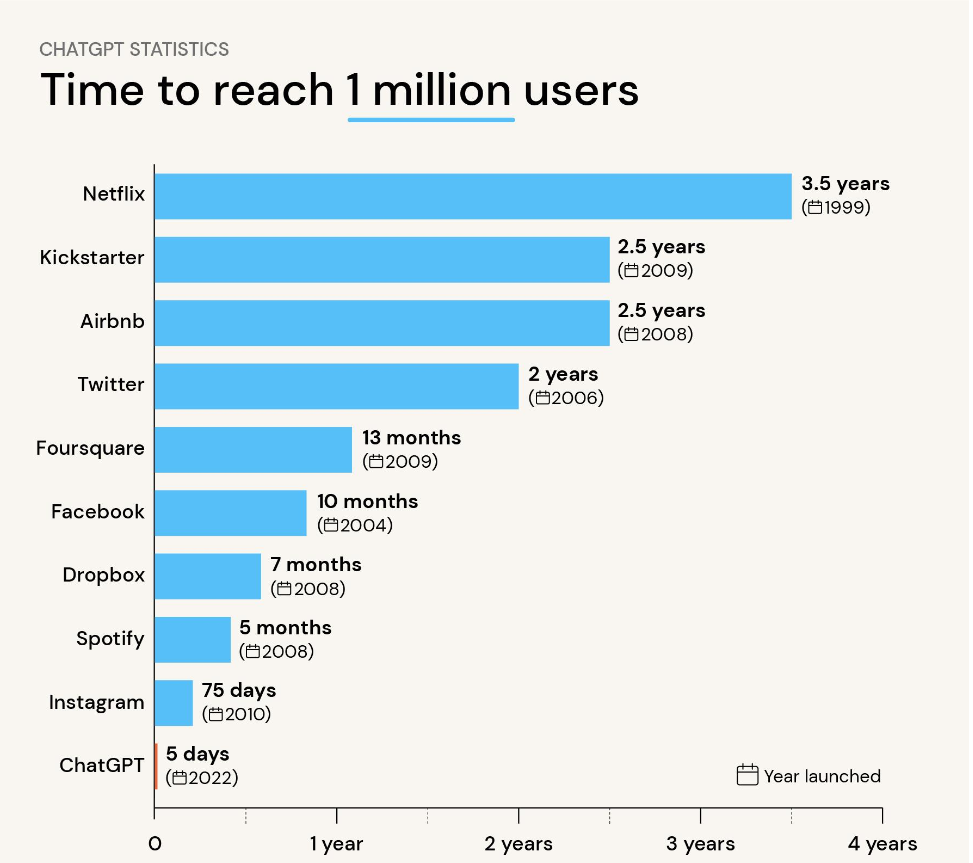
\includegraphics[width = 4in]{gpt_growth.png}
    \captionof{figure}{Tijd nodig tot 1 milioen gebruikers. \autocite{gpt_millie}}
    \label{fig:gpt_growth}
\end{center}

GPT-3 heeft een API die gebruikt kan worden.

\subsubsection{GPT-3.5}
GPT-3.5, een geüpgradede versie van het GPT-3-model, biedt geavanceerdere taalbegrip- en generatiecapaciteiten in vergelijking met zijn voorganger. De verbeteringen in GPT-3.5 stellen het model in staat om een breder scala aan complexe taken uit te voeren en betere resultaten te leveren in verschillende toepassingsgebieden, zoals tekstclassificatie, sentimentanalyse, tekstgeneratie en contextueel begrip \autocite{gpt_nappier, gpt_cn}. \\

\autocite{gpt_nappier} bespreken de technische aspecten van GPT-3.5 en de belangrijkste verschillen tussen GPT-3 en GPT-3.5. Een van de opmerkelijke verbeteringen in GPT-3.5 is het vermogen om context beter te begrijpen en relevante tekst te genereren op basis van die context. Dit is vooral belangrijk in taken waarbij contextuele informatie cruciaal is voor het begrijpen en genereren van geschikte antwoorden of voortzettingen van een tekst. \\

Een ander belangrijk aspect van GPT-3.5 is de verbeterde efficiëntie en prestaties. GPT-3.5 maakt gebruik van geoptimaliseerde architecturen en trainingsmethoden om de modelgrootte en computatievereisten te verminderen zonder concessies te doen aan de prestaties. Dit maakt het model toegankelijker en bruikbaarder voor een breder scala aan toepassingen en apparaten \autocite{gpt_nappier}. \\

\autocite{gpt_cn} verkennen de toepassingsmogelijkheden van GPT-3.5 en presenteren verschillende casestudy's die de prestaties en effectiviteit van het model aantonen. Ze onderzoeken het gebruik van GPT-3.5 in diverse domeinen, zoals het genereren van nieuwsartikelen, samenvatten van teksten, het beantwoorden van vragen op basis van tekst en het genereren van code. \\

Ondanks de goede prestaties van GPT-3.5, zijn er nog steeds uitdagingen en beperkingen die moeten worden aangepakt. In \autocite{gpt_cn} worden enkele van deze problemen besproken, zoals het genereren van irrelevante of onjuiste informatie (hallucineren), gevoeligheid voor vooroordelen in de trainingsdata en het vermogen om lange teksten te genereren zonder af te dwalen van het onderwerp. Toekomstig onderzoek zou zich kunnen richten op het verbeteren van deze aspecten en het ontwikkelen van methoden om de modelprestaties verder te verfijnen.\\

GPT-3.5 heeft een API die gebruikt kan worden onder de naam gpt-3.5-turbo. 

\subsubsection{GPT4}
GPT-4, de opvolger van GPT-3.5, is een nog geavanceerder transformer-gebaseerd taalmodel dat verder bouwt op de successen en verbeteringen van zijn voorgangers. GPT-4 biedt aanzienlijke verbeteringen op het gebied van natuurlijke taalverwerking, tekstgeneratie en begrip, evenals efficiëntie en bruikbaarheid \autocite{gpt_openai, gpt_micai}. \\

Een belangrijk kenmerk van GPT-4 is het vermogen om nog nauwkeuriger en coherenter menselijke taal te genereren en te begrijpen. Hierdoor kan GPT-4 beter presteren in verschillende toepassingsgebieden, zoals tekstclassificatie, sentimentanalyse, tekstgeneratie, contextueel begrip en vele anderen \autocite{gpt_micai}. \\

\autocite{gpt_cn} onderzoeken de technische aspecten en verbeteringen van GPT-4 ten opzichte van GPT-3.5. Ze benadrukken de geoptimaliseerde architecturen en trainingsmethoden die in GPT-4 zijn geïmplementeerd, waardoor het model betere prestaties kan leveren zonder dat dit ten koste gaat van de efficiëntie. Deze verbeteringen maken GPT-4 toegankelijker en bruikbaarder voor een breder scala aan toepassingen en apparaten. \\

Binnen het onderzoek van Microsoft \autocite{gpt_micai} toont men aan dat GPT-4 vormen van algemene intelligentie vertoont. Dit blijkt uit de kerncapaciteiten, zoals redeneren, creativiteit en deductie, expertise op verschillende onderwerpen, en de verscheidenheid aan taken die het kan uitvoeren. Hoewel er nog veel werk te doen is om een volledige AGI (Artificial General Intelligence) te creëren, wordt benadrukt dat het definiëren van intelligentie, AI en AGI complex en controversieel is en dat er geen definitieve definitie bestaat. Het onderzoek suggereert dat toekomstig werk op het gebied van GPT-4 en vergelijkbare systemen zich kan richten op het verkennen van nieuwe toepassingen en domeinen en het begrijpen van de mechanismen en principes die aan hun intelligentie ten grondslag liggen. \\

Naast de prestaties van GPT-4 hebben Elon Musk en andere experts opgeroepen tot een tijdelijke stop van Large Language Models (LLM) zoals GPT-4 kunnen overtreffen, vanwege potentiële risico's en onvoorziene gevolgen die dergelijke geavanceerde systemen met zich mee kunnen brengen zonder \autocite{reuters_musk}. 
 
\section{AI-gegenereerde kunst: tools en voorbeelden}
\subsection{ Midjourney}
Midjourney is een organisatie die met behulp van discord kunstwerken kan genereren, zo kun je een prompt sturen in de chat en krijg je verschillende kunstwerken te zien op basis van je prompt, indien je tevreden bent met de resultaten kun je de foto in hoge resultatie downloaden. Indien niet, kun je de beste van de X-aantal resultaten selecteren en hierop nieuwe resultaten laten genereren. 

\begin{center}
    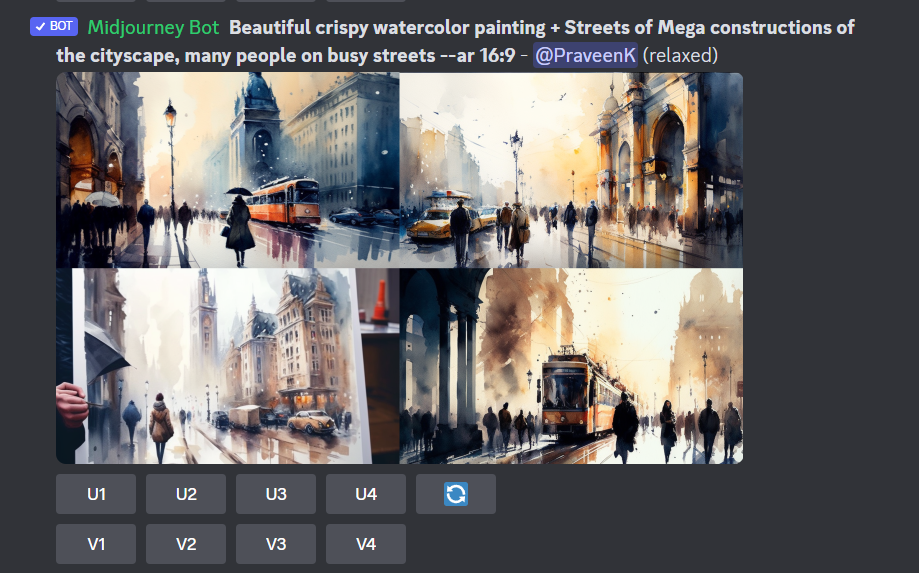
\includegraphics[width = 4in]{midjourney_ex.png}
    \captionof{figure}{Voorbeelden van AI-gegenereerde kunstwerken met behulp van Midjourney.}
    \label{fig:midjourney_ex.png}
\end{center}

Midjourney heeft geen API die we kunnen gebruiken.

\subsection{ Dall-E}
Dall-E kan gebruikt worden op de website om kunstwerkente generen maar met extra functionaliteiten vergeleken met midjourney. Dall-E laat het toe om foto's te editen en varianties van een kunstwerk te vragen. Met editen kun je een plaats markeren op het gegenereerde resultaat en hierop een nieuwe promp laten genereren, op deze manier kun je bepaalde dingen aanpassen of nieuwe attributen laten genereren op het kunstwerk. \\

Hieronder vindt u het resultaat gegenereerd op de prompt: ``Painted by Dali: Taiwan targeted by China'.' \\

\begin{figure}[h!]
    \centering
    \begin{tabular}{llll}
        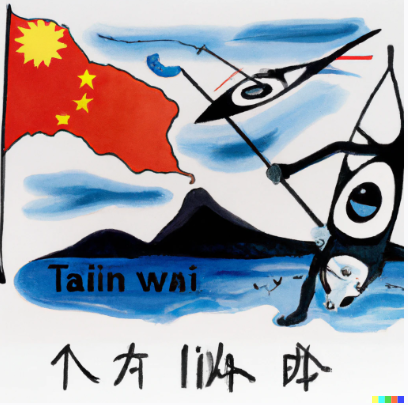
\includegraphics[width = 1.5in]{dall-e_ex1.png} &
        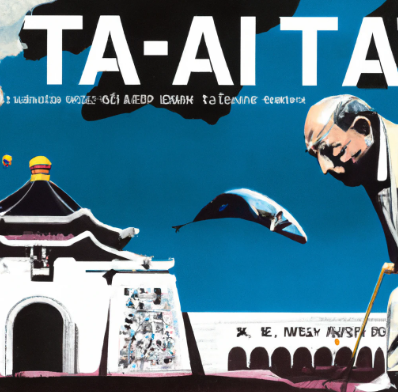
\includegraphics[width = 1.5in]{dall-e_ex2.png} \\
        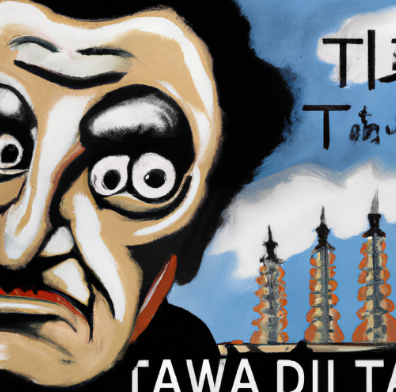
\includegraphics[width = 1.5in]{dall-e_ex3.png} &
        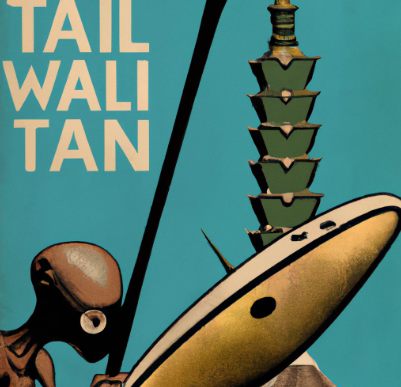
\includegraphics[width = 1.5in]{dall-e_ex4.png}
    \end{tabular}
    \caption{Voorbeelden van AI-gegenereerde kunstwerken met behulp van Dall-E.}
    \label{fig:examples}
\end{figure}


 Bovenstaande functionaliteiten worden ook aangeboden binnen de API van OpenAI.
\pagebreak

\subsection{Stable Diffusion}
Met Stable Diffusion kun je 1-4 kunstwerken laten genereren. \\

Hieronder vind u het resultaat gegenereerd op de prompt:  ``Painted by Van Gogh: War in Russia, food crisis in Asia.''

\begin{figure}[h!]
    \centering
    \begin{tabular}{llll}
        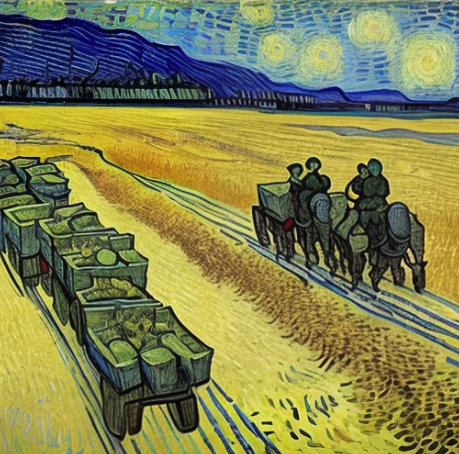
\includegraphics[width = 1.5in]{sd_ex1.png} &
        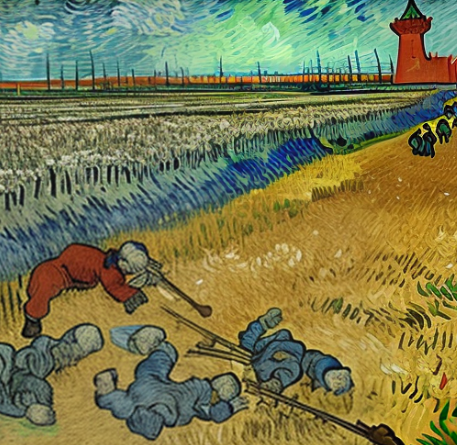
\includegraphics[width = 1.5in]{sd_ex2.png} \\
        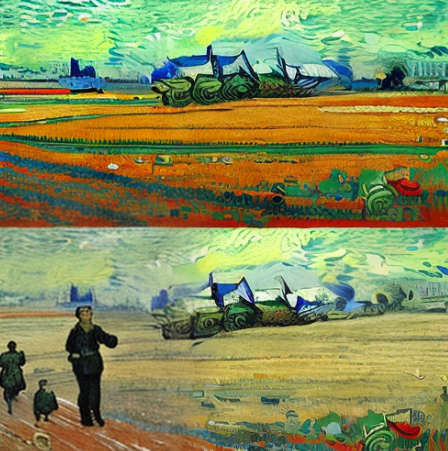
\includegraphics[width = 1.5in]{sd_ex3.png} &
        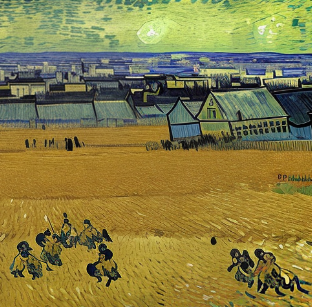
\includegraphics[width = 1.5in]{sd_ex4.png}
    \end{tabular}
    \caption{Voorbeelden van AI-gegenereerde kunstwerken met behulp van Stable Diffusion.}
    \label{fig:examples}
\end{figure}

Stable Diffusion heeft een API waarvan gebruik van gemaakt kan worden. \\

\pagebreak

\subsection{Toepassingen}
Binnen deze subsectie bespreek ik enkele toepassingen die gebruik maken van de eerder vermelde tools in punt 2.1/2.2 en 2.3.

\subsubsection{NFT's}
Een non-fungible token, beter bekend als een NFT, is een uniek digitaal object op een blockchain, meestal verbonden met speciale digitale content zoals foto's of muziek. Ze hebben een gigantische markt opgebouwd, waar individuele NFT's een waarde van miljoenen dollars kunnen bereiken \autocite{nft_whatisit}. \\

LLM's hebben het potentieel om de markt te verstoren op een manier die het menselijke aspect van NFT's kan wegnemen. In plaats van kunstenaars en creatievelingen die unieke digitale content maken, kunnen we een toekomst zien waarin AI de 'creator' wordt, wat de menselijke inspanning, creativiteit en originaliteit die traditioneel geassocieerd worden met kunst kan ondermijnen. 

\subsubsection{Graphic Design}
Binnen het domein van graphic design kunnen AI-tools zoals DALL-E en StyleGAN worden ingezet voor verschillende toepassingen. Zo kunnen ze bijvoorbeeld worden gebruikt om nieuwe verpakkingen, zoals cornflakesdozen, te ontwerpen door unieke en aantrekkelijke ontwerpen te genereren op basis van bestaande stijlen en trends.  \\

Daarnaast kunnen ze bedrijven helpen bij het creëren van opvallende en herkenbare logo's door verschillende concepten te genereren op basis van tekstbeschrijvingen of bestaande ontwerpelementen. 

\subsubsection{Webdevelopers}
Voor frontend webdevelopers kunnen AI-tools zoals Midjourney bijzonder handig zijn bij het opdoen van inspiratie voor het ontwerpen van websites. Door bijvoorbeeld aan Midjourney een prompt te geven zoals "Beautiful landing page Blissful state of mind, Natural healing techniques, Yoga, Meditation, ui, ux, elementor, wordpress, simple, minimalistic, aesthetics" \ref{fig:frontendwebdev_ex}, kan de AI-tool een reeks ontwerpen en concepten genereren die passen bij de gegeven beschrijving. Dit helpt webdevelopers om ideeën op te doen en hun creativiteit te stimuleren bij het bouwen van unieke en aantrekkelijke websites.

\begin{center}
    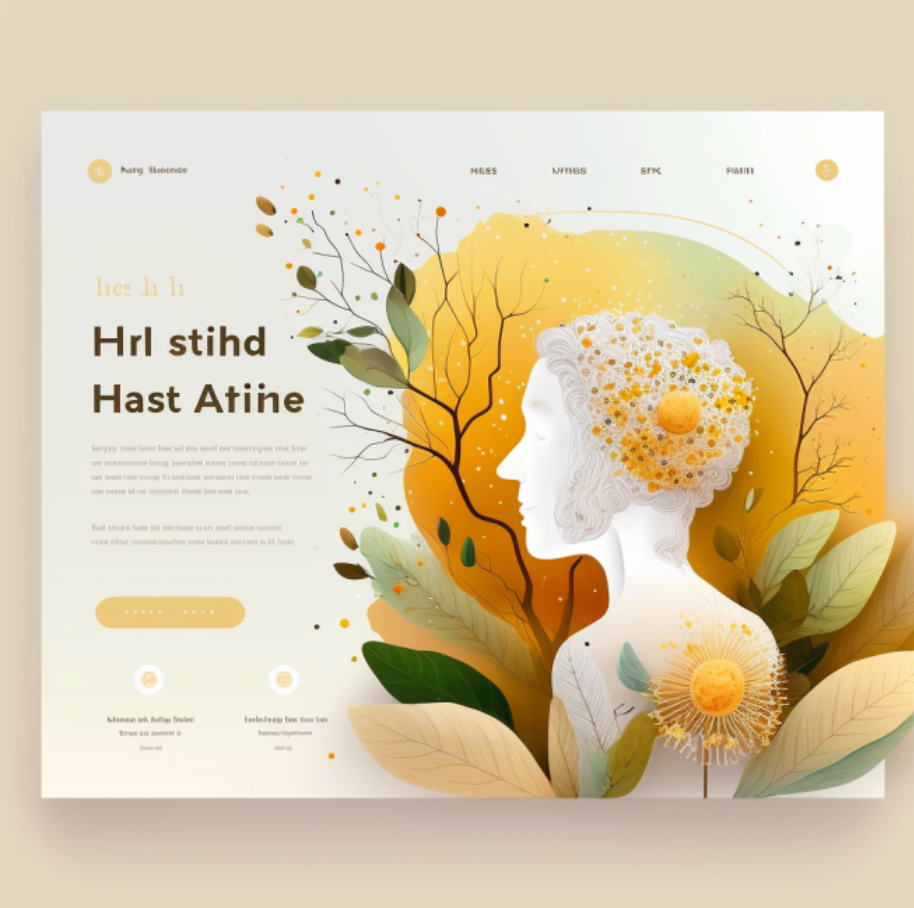
\includegraphics[width = 4in]{frontendwebdev_ex}
    \captionof{figure}{Voorbeeld: Landingspagina op basis van een prompt in Midjourney.}
    \label{fig:frontendwebdev_ex}
\end{center}


\section{Webscraping}
Webscraping is een krachtige techniek die gebruikt kan worden om tekstuele input te verzamelen voor het genereren van kunstwerken. Met webscraping kunnen gegevens van websites worden geëxtraheerd en gebruikt worden als input voor generatieve AI-algoritmen om kunstwerken te genereren. \\
 
Een belangrijke overweging bij het gebruik van webscraping voor het genereren van kunstwerken is het respecteren van de regels en beperkingen van de websites die worden gescraped. Websites kunnen bijvoorbeeld beperkingen opleggen via het robots.txt-bestand, dat aangeeft welke delen van de website geopend kunnen worden voor scraping. Het is belangrijk om deze regels te respecteren en alleen gegevens te verzamelen waarvoor toestemming is verleend. \\

Belangrijke zaken waarmee er rekening gehouden moet worden om een scraper te creeëren volgens \autocite{BIO2014}:

\begin{itemize}
    \item \textbf{Toegang krijgen tot de site:} De webscraper maakt verbinding met de doelwebsite via het HTTP-protocol en houdt rekening met verzoeksmethoden zoals GET en POST. Daarnaast moet de 'User-Agent' correct worden ingesteld.
    \item \textbf{HTML-Parsen en de inhoud extraheren:} De scraper moet in staat zijn om de HTML-structuur van de webpagina te begrijpen en de relevante gegevens te extraheren. Dit kan worden bereikt met behulp van reguliere expressies, HTML-parsing bibliotheken of op selectors gebaseerde talen zoals XPath en CSS-selector syntax.
    \item \textbf{Output:} De geëxtraheerde gegevens moeten worden omgezet in een gestructureerde weergave die geschikt is voor verdere analyse en opslag, zoals in-memory datastructuren of tekstgebaseerde bestandsformaten zoals XML of CSV.
\end{itemize}

\subsection{Ethische aspecten}
\label{subsection:scraper-ethische-aspecten}
Bij het uitvoeren van webscraping-activiteiten is het van belang om ethische overwegingen in acht te nemen. Webscraping kan verschillende ethische uitdagingen met zich meebrengen, zoals het respecteren van de privacy van gebruikers en het naleven van de regels en beperkingen van websites. Hier zijn enkele belangrijke ethische aspecten volgens \autocite{scrape_ethics} om rekening mee te houden tijdens het ontwikkelen van de scraper: 

\begin{itemize}
    \item \textbf{Privacy en persoonlijke gegevens:} Het is essentieel om geen persoonlijke identificeerbare informatie of gevoelige gegevens te verzamelen zonder de toestemming van de gebruikers of de website-eigenaren.
    \item \textbf{Auteursrecht en intellectuele eigendom:} Het is belangrijk om de regels en beperkingen van websites te respecteren met betrekking tot het gebruik en de reproductie van hun inhoud.
    \item \textbf{Serverbelasting:} Webscraping kan de serverbelasting van websites verhogen, vooral als grote hoeveelheden gegevens worden opgevraagd of als frequent en intensief scraping plaatsvindt. Dit kunnen we vermijden door een wachttijd te simuleren na elke request. 
\end{itemize}

\subsection{BeautifulSoup4}
BeautifulSoup4 (BS4) is een populaire Python-bibliotheek voor webscraping die het eenvoudig maakt om gegevens van webpagina's te verkrijgen en te verwerken \autocite{BIO2014, BSFOR2015}. \\

Het biedt een intuïtieve en eenvoudige manier om HTML- en XML-documenten te parseren en gegevens eruit te extraheren. Met BeautifulSoup4 kunnen ontwikkelaars elementen selecteren op basis van tags, klassen, ids en andere attributen. Ze kunnen ook door de hiërarchie van de HTML-structuur navigeren en de gewenste gegevens extraheren. \\

De officiële documentatie van BeautifulSoup4 is een waardevolle bron van informatie en richtlijnen voor het gebruik van de bibliotheek. Het bevat gedetailleerde uitleg, voorbeelden en referenties naar de verschillende functies en methoden van BeautifulSoup4. 
De documentatie is beschikbaar op de volgende website: \autocite{BS4Documentation}. \\


\section{De uitdagingen en beperkingen van AI-gegenereerde kunst}
AI-gegenereerde kunst brengt verschillende uitdagingen en beperkingen met zich mee, die invloed hebben op de creativiteit, originaliteit en interpretatie van de gegenereerde kunstwerken en dus ook het onderzoek zelf.

\subsection{Creativiteit}
Een van de belangrijkste uitdagingen bij AI-gegenereerde kunst is het stimuleren van creativiteit. Hoewel AI in staat is om grote hoeveelheden gegevens te analyseren en patronen te herkennen, mist het vaak de menselijke verbeeldingskracht en intuïtie die nodig zijn voor het creëren van originele en innovatieve kunstwerken. AI-algoritmen zijn gebaseerd op bestaande gegevens en modellen, waardoor ze vaak geneigd zijn om bestaande stijlen en trends te repliceren in plaats van iets volledig nieuws te creëren. Het uitdagen van AI om buiten de gebaande paden te denken en echt unieke kunstwerken te genereren, blijft een grote uitdaging.

\subsection{Originaliteit}
Een andere beperking van AI-gegenereerde kunst is de kwestie van originaliteit. Omdat AI-systemen zijn getraind op bestaande datasets, bestaat het risico dat ze onbedoeld bestaande kunstwerken of ideeën reproduceren zonder voldoende originaliteit toe te voegen. Dit kan leiden tot het genereren van kunstwerken die sterk lijken op bestaande werken of het schenden van auteursrechten. Het waarborgen van voldoende originaliteit in AI-gegenereerde kunst vereist een zorgvuldige afweging tussen het gebruik van bestaande gegevens voor training en het aanmoedigen van nieuwe, unieke expressie.

\subsection{Interpretatie}
Een uitdaging bij het omgaan met AI-gegenereerde kunst is de interpretatie ervan. Omdat kunstwerken vaak worden geassocieerd met emotie, betekenis en subjectiviteit, kan de interpretatie van AI-gegenereerde kunstwerken een uitdaging zijn. Het ontbreekt AI vaak aan de menselijke context en begrip om diepere betekenissen en nuances in kunstwerken te begrijpen. Dit kan resulteren in kunstwerken die voor mensen moeilijk te interpreteren zijn of die niet de gewenste emotionele impact hebben. Het betrekken van menselijke interactie en interpretatie bij AI-gegenereerde kunst kan helpen om deze uitdaging aan te pakken en een meer gelaagde en betekenisvolle ervaring te creëren.

Het is belangrijk om deze uitdagingen en beperkingen in gedachten te houden bij het ontwikkelen en evalueren van AI-gegenereerde kunst. Door voortdurend te streven naar creativiteit, originaliteit en begrijpelijke interpretatie, kunnen we de potentie van AI benutten om nieuwe vormen van artistieke expressie te verkennen en te ontwikkelen.

%%=============================================================================
%% Methodologie
%%=============================================================================

\chapter{\IfLanguageName{dutch}{Methodologie}{Methodology}}%
\label{ch:methodologie}

%% TODO: Hoe ben je te werk gegaan? Verdeel je onderzoek in grote fasen, en
%% licht in elke fase toe welke stappen je gevolgd hebt. Verantwoord waarom je
%% op deze manier te werk gegaan bent. Je moet kunnen aantonen dat je de best
%% mogelijke manier toegepast hebt om een antwoord te vinden op de
%% onderzoeksvraag.
\section{Inleiding}
Het onderzoek begint met een grondige literatuurstudie die te vinden is in Hoofdstuk 2. Deze literatuurstudie bepaalt de onderwerpen waarop dit onderzoek zich zal richten en onderzoekt enkele belangrijke en veelvoorkomende webscraping- en AI-modellen die momenteel beschikbaar zijn.  \\

\section{Fases}
\begin{itemize}
    \item \textbf{Fase 1}: Ontwikkelen van een webscraper die in staat is om de website, titel op een correct en gestructureerde manier te verzamelen. 
    \item \textbf{Fase 2}: Prompt genereren met GPT met behulp van de verzamelde artikels. 
    \item \textbf{Fase 3}: Genereren van een kunstwerk met DALL-E op basis van de prompt uit vorige fase 2.
\end{itemize} 

\section{Onderverdeling}

Hoofdstuk \ref{ch:proof-of-concept}  beschrijft de proof-of-concept van het onderzoek. Het bevat de ontwikkeling van de webscraper in fase 1 en het gebruik van de verzamelde artikelen als input voor het GPT en DALL-E model in fase 2 en 3. Er zal uitgelegd worden hoe de gegenereerde prompts dienen als basis voor het genereren van schilderijen met behulp van DALL-E. Het doel van dit hoofdstuk is om de implementatie en werking van de applicatie aan te tonen op basis van de verkregen informatie uit hoofdstuk \ref{ch:stand-van-zaken}.  \\

Hoofdstuk beschrijft \ref{ch:evaluatieproces} de evaluatieproces van het gegenereerde kunstwerk. In dit hoofdstuk wordt er een evaluatieproces beschreven dat de te geïnterpreteerde waarde van het schilderij achterhaalt. Dit zal gedaan worden aan de hand van een turingtest waar we de deelnemers zullen bevragen om een boodschap uit een schilderij te halen. (of een nieuwsartikel hieraan te koppelen) Met behulp van deze turingtest kunnen we bepalen of AI in staat is om de boodschap van het nieuws over te brengen.



\chapter{\IfLanguageName{dutch}{proof-of-concept}{proof-of-concept}}%
\label{ch:proof-of-concept}
\section{Inleiding}
In dit hoofdstuk bespreken we de implementatie van het proof-of-concept. We bespreken elke fase van het proces in detail en de implementatie van de bijbehorende componenten toelichten. Hierbij zullen we ook de uitkomsten van elke fase beschrijven en hoe deze kunnen gebruikt worden in de volgende fase. 

\section{Webscraper}
\subsection{Algemene Eisen}
Binnen de algemene eisen zal de webscraper voldoen aan de ethische aspecten \ref{subsection:scraper-ethische-aspecten} die eerder werden beschreven. Dit betekent dat de scraper de regels en richtlijnen van de gescrapte websites zal respecteren en zich zal houden aan eventuele beperkingen zoals vermeld in het robots.txt-bestand. Hierdoor wordt ervoor gezorgd dat de scrapingactiviteiten op een ethisch verantwoorde manier worden uitgevoerd. \\

Daarnaast zal de webscraper in staat zijn om verschillende websites te scrapen, met de focus op het verzamelen van de frontpage-inhoud. Specifiek zal de scraper de eerste 20 items van de frontpage van elke website verzamelen. \\

De webscraper zal twee bekende nieuwsbronnen scrapen, namelijk HLN en DeMorgen.

\subsection{Verkenning}
Alvorens we de webscraper kunnen implementeren, is het nodig om de DOM-structuur \footnote{De DOM-structuur (Document Object Model) is een hiërarchische representatie van een HTML- of XML-document.} van beide websites te bekijken en een patroon hierin te herkennen. 
\subsubsection{HLN}
Op de startpagina van HLN kunnen we zien (figuur \ref{fig:hln_frontpage}) dat elk nieuwsartikel zich bevindt binnen een article-tag bevindt. De eerste subtag is een a-tag met hierin de href naar het artikel. \\ Deze href zal belangrijk zijn om de datum te valideren en de titel te extraheren. We moeten deze dus opslaan. 

\begin{center}
    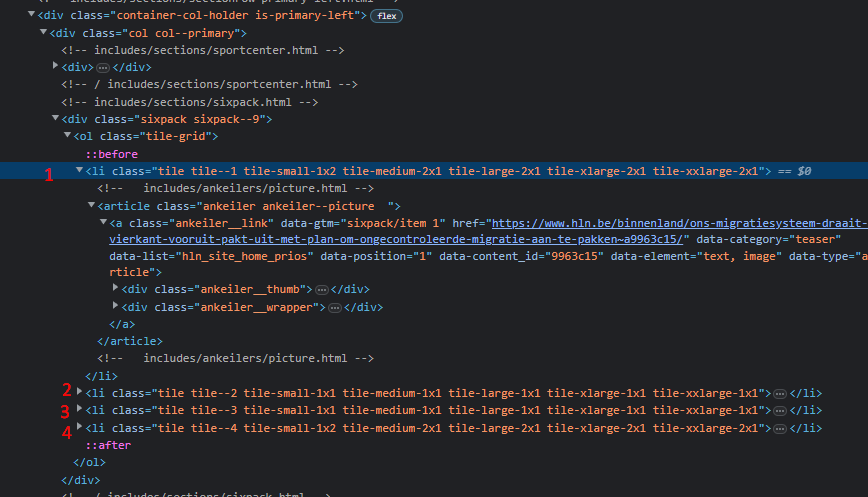
\includegraphics[width = 6in]{hln_frontpage2.png}
    \captionof{figure}{DOM-structuur van de startpagina van HLN met hierop verschillende nieuwsartikels op aangeduid.}
    \label{fig:hln_frontpage}
\end{center}

Als we vervolgens gaan kijken naar de DOM-structuur van een artikel, zien we dat de titel weergegeven wordt binnen een header-tag met als class 'article\_\_header' deze titel heeft als class 'article\_\_title'. De datum wordt weergegeven binnen een time-tag met datetime als value en class 'article\_\_time'. De datum is ook opgemaakt in een bepaald formaat, dd-mm-yy, hh:mm. Deze gegevens zijn essentieel voor de scraper. In figuur \ref{fig:hln_article} vind je dit terug. \\

\begin{center}
    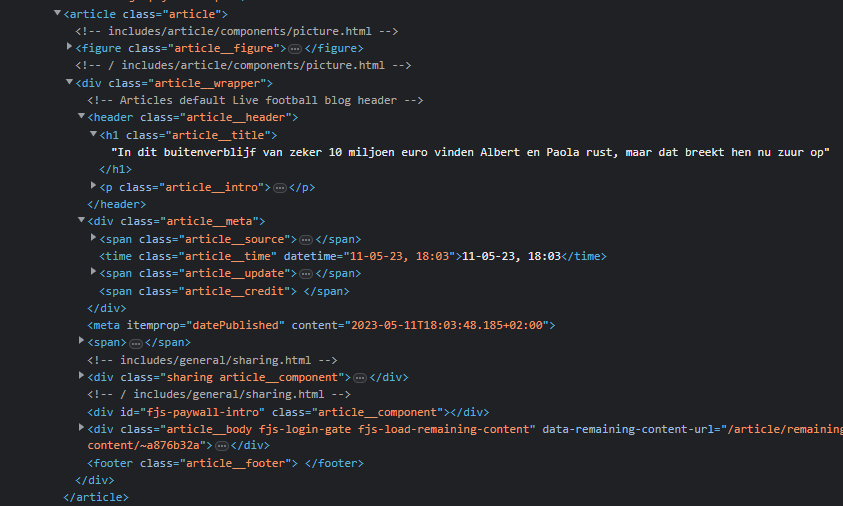
\includegraphics[width = 6in]{hln_article1.png}
    \captionof{figure}{DOM van een artikel op HLN.}
    \label{fig:hln_article}
\end{center}

\subsubsection{De Morgen}
De structuur van de artikels op de startpagina van De Morgen is vergelijkbaar met die van HLN. Zoals te zien is in figuur \ref{fig:demorgen_frontpage}, worden de artikels ook weergegeven binnen een article-tag, alleen is bij de morgen de tweede child de a-tag ten opzichte van HLN.

\begin{center}
    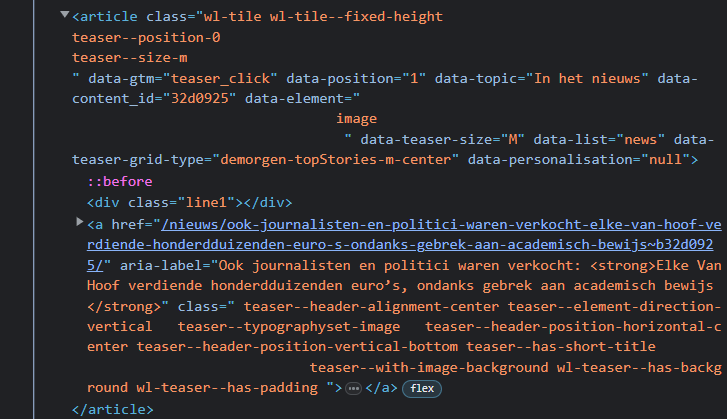
\includegraphics[width = 6in]{demorgen_frontpage2.png}
    \captionof{figure}{DOM van een artikel op De Morgen.}
    \label{fig:demorgen_frontpage}
\end{center}

Bij het doorklikken op een willekeurig artikel zien we dat de DOM-structuur vergelijkbaar is, maar niet exact hetzelfde qua structuur. In figuur \ref{fig:demorgen_article} zie je de DOM.

\begin{center}
    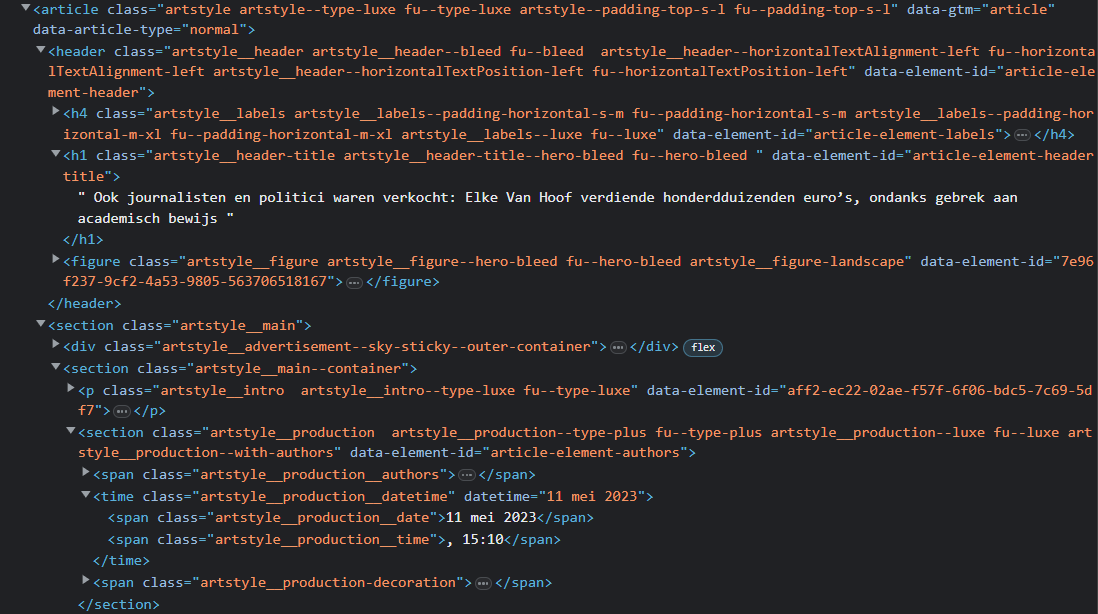
\includegraphics[width = 6in]{demorgen_article.png}
    \captionof{figure}{DOM van een artikel op De Morgen.}
    \label{fig:demorgen_article} 
\end{center}

Nu dat we deze informatie hebben. Kunnen we beginnen aan de implementatie van de scraper. 

\subsection{Implementatie}
\subsubsection{Thread-safe Dictionary}
Om ervoor te zorgen dat de gescrapete data veilig wordt opgeslagen, beginnen we de implementatie met het maken van een thread-safe dictionary.
\begin{pythoncode}{../../../workspace/paper/scraper/util/volatileDictionary.py}
Deze thread-safe dictionary zal de opslag van de gescrapete data beheren en ervoor zorgen dat er geen problemen ontstaan tijdens het wegschrijven van de gescrapete data.
\end{pythoncode}

\subsubsection{Abstracte Thread}
Voordat we de specifieke threads implementeren, maken we eerst een AbstractThread-klasse die de methoden definieert die door de specifieke threads zullen worden gebruikt.

De AbstractThread-klasse bevat het volgende:

\begin{itemize}
    \item \textbf{Constructor}: Initialiseert de gemeenschappelijke eigenschappen die vereist zijn door de specifieke threads.
    \item \textbf{Methoden}: Definieert de gemeenschappelijke methoden die door de specifieke threads zullen worden gebruikt.
\end{itemize}

Laten we de \textbf{constructor} van de AbstractThread-klasse bespreken:

\begin{pythoncode}{../../../workspace/paper/abstractThreadCTR.py}
    In de constructor initialiseren we de gemeenschappelijke eigenschappen die vereist zijn door de specifieke threads. Deze eigenschappen omvatten:
\end{pythoncode}

    \begin{itemize}
        \item \textbf{dict}: De thread-safe dictionary die gebruikmaakt van dependency injection en geïnitialiseerd wordt.
        \item \textbf{limit}: De maximum waarde waarvan de artikels ouder moeten zijn.
        \item \textbf{articles}: De artikels die moeten worden verwerkt.
        \item \textbf{dateformat}: Het formaat van de datum dat wordt weergegeven in de artikelen.
        \item \textbf{title\_tag, title\_class, time\_tag, time\_class}: De HTML klassen waar de relevante gegevens in voorkomt.
        \item \textbf{base\_url}: De URL waarop de scraper moet starten.
        \item \textbf{routes}: De routes waarop de scraper toegestaan is te scrapen, rekening houdend met robots.txt terug te vinden op punt \ref{ch:liter_webscraping}.
        \item \textbf{headers}: De headers die aan de verzoeken worden toegevoegd om toegang te krijgen tot de website.
        \item \textbf{current}: Het momenteel verwerkte artikel.
        \item \textbf{article\_link}: De link van het huidige artikel dat overeenkomt met de opgegeven routes en momenteel wordt gescraped. \\
    \end{itemize}

Daarnaast bevat de AbstractThread-klasse ook verschillende methoden die het scrapen mogelijk maken. Laten we deze methoden bespreken:

\begin{pythoncode}{../../../workspace/paper/abstractThreadONSTART.py}
 Deze methode stuurt een initiële aanvraag naar de base\_url om de eerste 20 artikelen op te halen.
\end{pythoncode}

\begin{pythoncode}{../../../workspace/paper/abstractThreadSTARTSCRAPING.py}
Deze methode voert de on\_start()-methode uit, die de initiële artikelen ophaalt. Vervolgens gaat het door met het scrapen van artikelen zolang er artikelen in de lijst zijn. Elk artikel wordt gecontroleerd met behulp van de should\_scrape\_article()-methode en als het aan de voorwaarden voldoet, wordt het gescraped met behulp van de scrape\_article()-methode.
\end{pythoncode}

\begin{pythoncode}{../../../workspace/paper/abstractThreadSHOULDSCRAPE.py}
Deze methode controleert of de URL van een artikel overeenkomt met een van de opgegeven routes. Als dit het geval is, wordt de article\_link ingesteld en wordt True geretourneerd om aan te geven dat het artikel moet worden gescraped.
\end{pythoncode}

\begin{pythoncode}{../../../workspace/paper/abstractThreadSCRAPE.py}
    Deze methode haalt de inhoud van de article\_link op met behulp van een GET-verzoek en de opgegeven headers. Vervolgens worden de datum en titel geëxtraheerd op basis van de opgegeven HTML-klassen. Als de geëxtraheerde datum vandaag is, wordt de append\_to\_dict()-methode aangeroepen om het artikel op te slaan in de thread-safe dictionary. \\
    
    Na elke request naar een bepaald artikel wordt er een korte sleep geïmplementeerd zodat we niet overdrijven in het aantal request dat we versturen om de server niet te overbelasten zoals besproken in punt \ref{subsection:scraper-ethische-aspecten}. \\
\end{pythoncode}

De AbstractThread-klasse biedt een basis voor het implementeren van de specifieke threads.

\subsubsection{HLNThread}
    De HLNThread wordt aangemaakt met de volgende code:
    
\begin{pythoncode}{../../../workspace/paper/hlnThread.py}
    De HLNThread wordt geïnitialiseerd met de specifieke eigenschappen die vereist zijn voor het scrapen van artikelen op de HLN-website. De base\_url is "https://www.hln.be" en de routes zijn ["/buitenland", "/binnenland", "/vtm-nieuws"]. De HTML-klassen voor de titel en de datum worden ook opgegeven.
\end{pythoncode}

\subsubsection{De Morgen Thread}
    De DeMorgenThread wordt aangemaakt met de volgende code:

\begin{pythoncode}{../../../workspace/paper/deMorgenThread.py}
    DeMorgenThread wordt geïnitialiseerd met de specifieke parameters die vereist zijn in de AbstractThread voor het scrapen van de website. De base\_url is 'https://www.demorgen.be' en de routes moeten nog worden toegevoegd, afhankelijk van de specifieke routes op de website van De Morgen doen we dit binnenin de on\_start()-methode om zo steeds de up-to-date routes te hebben. De HTML-klassen voor de titel en de datum worden ook opgegeven.
\end{pythoncode}

\subsubsection{Uitvoering}
Om dit nu allemaal te kunnen uitvoeren zullen we een scraper klasse maken, die de verschillende threads initializeerd en de uitkomst hiervan retourneerd. De implementatie hiervan is als volgt: 
\begin{pythoncode}{../../../workspace/paper/scraper.py}
    Hiervoor wordt gebruikt gemaakt van een ThreadPoolExecutor om de threads te runnen en de uitkomst hiervan als future terug te krijgen. Als uitkomst hiervan wordt de dictionary ge-retourneerd.
\end{pythoncode}

\subsection{Uitkomst}
Om de uitkomst hiervan te testen, maken we een nieuw bestand aan genaamd \_\_main\_\_.py en gebruiken we dit bestand als het startpunt van onze applicatie. Hieronder vind je de inhoud van \_\_main\_\_.py:
\begin{pythoncode}{../../../workspace/paper/scraperMain.py}
In de main functie starten we het scrapingproces door de start\_scraping()-methode aan te roepen. De gescrapete gegevens worden opgeslagen en geprint op de console. \\

De start\_scraping functie initialiseert een VolatileDict object om de gescrapete gegevens op te slaan. Vervolgens maken we instanties van de specifieke threads en voegen we ze toe aan de lijst threads. We gebruiken een ThreadPoolExecutor om de threads parallel uit te voeren en slaan de resultaten op in de futures lijst. \\

Na het voltooien van alle threads halen we de gescrapete gegevens op met behulp van de output\_dict() methode van het VolatileDict object. Deze gegevens worden geretourneerd als het resultaat van de functie. \\

Dit is een basisimplementatie van het startpunt van de applicatie, die in volgende stappen wordt aangepast en uitgebreid.
\end{pythoncode}

Het resultaat van de scraper kun je terugvinden in bijlage.

\section{GPT}
\subsection{Inleiding}
Om GPT te kunnen gebruiken, zullen we de API van OpenAI gebruiken. Deze API kan prijzig zijn, vooral voor GPT-4. Daarom zullen we binnen dit onderzoek gebruik maken van GPT-3.5, wat neerkomt op ongeveer \$0.05 per verzoek \autocite{gpt_pricing}.

Volgens de API kan GPT verdergaan in een conversatie door gebruik te maken van een dialoog.

De implementatie zal ervoor zorgen dat we een conversatie starten met GPT en hem vragen om een prompt te retourneren, zoals: 'Thema en/of gevoel en/of onderwerp geschilderd door: ...'. We zullen hiervoor de OpenAI Python-bibliotheek gebruiken, die beschikbaar is op GitHub\footnote{\url{https://github.com/openai/openai-python}}.

\subsection{Implementatie}
\subsubsection{Configuratie}
Om de API te kunnen gebruiken, hebben we een API-sleutel nodig. Na het genereren van een sleutel op de website, kunnen we deze in een .env-bestand plaatsen en deze gebruiken in onze configuratie. Hieronder vind je de implementatie van de configuratie.
\begin{pythoncode}{../../../workspace/paper/openAI/util/config.py}
\end{pythoncode}

\subsubsection{RequestHandler}
Omdat we de API zullen gebruiken voor verschillende gebruiksscenario's, hebben we een RequestHandler nodig. Deze RequestHandler stelt de API-sleutel van OpenAI in en voert de verzoeken uit naar OpenAI. Hieronder vind je de code voor deze klasse.
\begin{pythoncode}{../../../workspace/paper/openairequesthandler1.py}
\end{pythoncode}

\subsubsection{ChatGPT}
Tot slot zullen we een klasse maken genaamd ChatGPT, die verantwoordelijk is voor alle communicatie met GPT. Deze klasse start een conversatie met GPT. Uiteindelijk ontvangt hij de gescrapete gegevens en retourneert hij de prompt voor DALL-E. Hieronder wordt de code geïllustreerd.
\begin{pythoncode}{../../../workspace/paper/openAI/chatgpt.py}
\end{pythoncode}

\subsection{Uitkomst}
We kunnen deze code nu testen door de volgende twee regels code toe te voegen aan het \_\_main\_\_.py-bestand.
\begin{pythoncode}{../../../workspace/paper/gptMain.py}
\end{pythoncode}
De uitkomst hiervan is zeer verschillend. Met de gescrapete gegevens die te vinden zijn in de uitkomst van de webscraper, krijg je telkens een andere uitkomst.

Hier is een voorbeeld van een conversatie:
\begin{drama}
    \Character{Applicatie:}{app}
    \Character{GPT-3.5:}{gpt}
    
    \appspeaks{ Ik zou graag een kunstwerk willen genereren met DALL-E gebaseerd op de hoogtepunten van vandaag. 
        Ik heb enkele artikels gevonden van vandaag, en deze gegroepeerd per url.
        Ik heb enkel de titel van het artikel opgeslaan.}
    
    \gptspeaks{Helaas ben ik als AI taalmodel niet in staat om toegang te krijgen tot het internet om webinhoud te scannen. Wanneer u toegang heeft tot de inhoud van de artikelen, kunt u deze naar mij sturen en kan ik proberen om op basis van deze informatie een kunstwerk te genereren met DALL-E.}
    
    \appspeaks{Welke artikels zijn er het belangrijkst volgens jou, rekeninghoudend met vorige criteria. 
        Hieronder vind je de artikels in json formaat, gegroepeerd per url van belangrijk naar minder belangrijk. <json data gescraped met webscraper>}
    
    
    \gptspeaks{Op basis van de beschikbare titels van de artikelen, zou ik de volgende groepering van hoogtepunt-artikelen aanbevelen:  
        \begin{itemize}
            \item{‘Ook aan hun kant ontploft er heel wat’: Oekraïne lijkt te dralen met zijn tegenoffensief.}
            \item{Poetins geheime bunkercomplex onder gigantisch paleis aan Zwarte Zee onthuld: zo ziet het eruit.}
            \item{VS zetten licht op groen voor training Oekraïense piloten in westerse gevechtsvliegtuigen.}
        \end{itemize}
Merk op dat deze groepering enkel gebaseerd is op de titels van de artikelen en dat deze niet noodzakelijk overeenkomen met de werkelijke gebeurtenissen of de inhoud van de artikelen. Ik raad je aan om de artikelen en hun inhoud te lezen om beter te begrijpen waarover ze gaan en om zelf een weloverwogen beslissing te nemen over welke gebeurtenissen je relevant vindt om in een kunstwerk te verwerken.}

    
    \appspeaks{Als je voor mij hier één kernzin kan uithalen; een samenvatting. Welke zou het dan zijn?}
    
    \gptspeaks{De kernboodschap van de artikelen is dat er zich tragische gebeurtenissen hebben voorgedaan, zoals dodelijke ongevallen, schietpartijen en conflicten tussen landen. Deze gebeurtenissen worden gekenmerkt door verlies, geweld en spanning. Een schilderij dat deze boodschap weerspiegelt, zou de emotionele impact en de donkere aspecten van deze gebeurtenissen kunnen benadrukken..}
    
    \appspeaks{Maak voor mij een kernboodschap op basis van voorgaand JSON. Houd de boodschap beperkt tot één artikel.}
    
    \gptspeaks{Op basis van de beschikbare artikelen in de gegeven JSON, zou ik de volgende kernboodschap aanbevelen: "Tragische gebeurtenissen markeren het verlies van mensenlevens en de schokkende realiteit van geweld'}
    
    \appspeaks{Ik zou dit nu graag laten genereren door dall-e om een kunstwerk te krijgen.
        Wat zou een goede prompt kunnen zijn die een kernboodschap weergeeft van de belangrijkste artikel, de boodschap moet goed overkomen.
        Vergeet geen stijl erbij te zeggen.}
    
    \gptspeaks{Een prompt die de kernboodschap van de artikels weergeeft en geschikt zou kunnen zijn voor een kunstwerk gegenereerd door DALL-E zou kunnen luiden: Een indringend kunstwerk dat de tragiek van verlies en het conflict tussen Rusland en Oekraine verbeeldt, in expressief realisme.}
    
    \appspeaks{Reageer enkel met een prompt die deze kernboodschap weergeeft en zet deze tussen quotes zet er ook bij door welke kunstenaar deze is geschilderd of in welke stijl. Gebruik maximum 75 karakters.}
    
    \gptspeaks{\textbf{''Expressief realistisch schilderij: verlies, conflict Rusland-Oekraïne."}}
    
    \appspeaks{Op basis van welke kernartikels heb je dit gehaald?}
    
    \gptspeaks{Dit kunstwerk is gebaseerd op de drie belangrijkste artikelen zoals eerder vermeld, namelijk het tegenoffensief van Oekraïne, Poetins geheime bunkercomplex aan de Zwarte Zee en VS die de training van Oekraïense piloten start. }
\end{drama}

    \noindent
    Op basis van de prompt kunnen we wel degelijk het nieuws herkennen van vandaag. Laten we kijken of dit nu ook een positief resultaat geeft binnen DALL-E.


\section{DALL-E}

\subsection{Inleiding}
Net als bij GPT maken we gebruik van de OpenAI Python-bibliotheek om DALL-E te benaderen. Met DALL-E kunnen we kunstwerken creëren die overeenkomen met de prompts gegenereerd door GPT.

\subsection{Implementatie}
Om kunstwerken te genereren met behulp van DALL-E, moeten we eerst de RequestHandler uitbreiden met een nieuwe methode om verzoeken te versturen via de openai library. Vervolgens definiëren we een klasse voor DALL-E, zodat we deze kunnen gebruiken in het 
\_\_main\_\_.py bestand. \\

We beginnen met het uitbreiden van de RequestHandler.

\subsubsection{Uibreiding van RequestHandler}
Om het verzoek te versturen, definiëren we een nieuwe methode generate\_image(self, prompt) die de prompt naar de API verzendt. We ontvangen de URL terug waar het kunstwerk te vinden is. Het eindresultaat ziet er als volgt uit:
\begin{pythoncode}{../../../workspace/paper/openAI/util/openairequesthandler.py}
\end{pythoncode}

\subsubsection{DALL-E}
Nu we het verzoek kunnen versturen, maken we een klasse DALL-E aan die deze methode zal uitvoeren binnen het  \_\_main\_\_.py-bestand. Hieronder vind je de implementatie:
\begin{pythoncode}{../../../workspace/paper/openAI/dalle.py}
\end{pythoncode}
    
\subsection{Resultaat}
Ten slotte breiden we het \_\_main\_\_.py-bestand uit met deze code, resulterend in de volgende code:
\begin{pythoncode}{../../../workspace/paper/__main__.py}
\end{pythoncode}
Om het resultaat te testen, gebruiken we de prompt: \emph{"Expressief realistisch schilderij: verlies, conflict Rusland-Oekraïne."}, verkregen uit de voorgaande implementatie, om met DALL-E een kunstwerk te genereren. \\

DALL-E genereert een URL waar we het kunstwerk kunnen bekijken. De onderstaande afbeelding toont het gegenereerde kunstwerk.

\begin{center}
    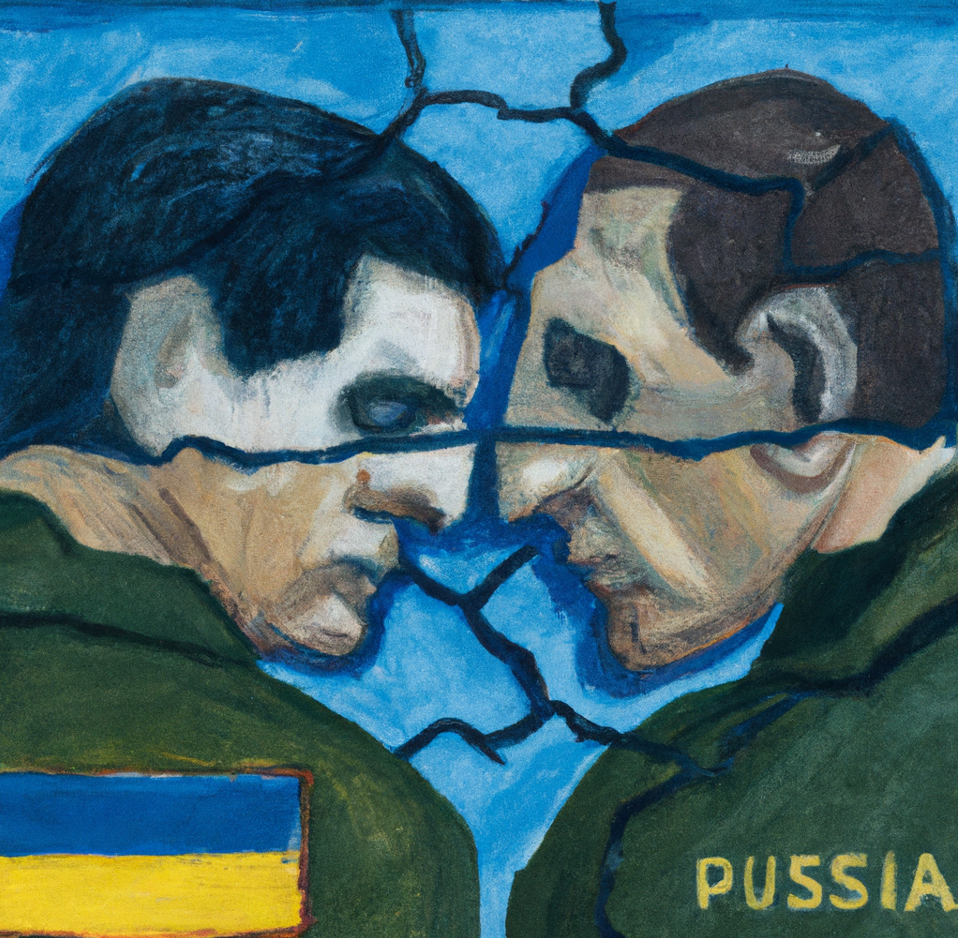
\includegraphics[width = 4in]{dall-e_result.png}
    \captionof{figure}{Kunstwerk gegenereerd met DALL-E en GPT met behulp van de gescrapete data in figuur 4.5}
    \label{fig:dall-e_result}
\end{center}

In het volgende hoofdstuk zullen we het resultaat van deze proof of concept gaan valideren om zo een antwoord te kunnen bieden op de vraag: Is AI geavanceerd genoeg om kunstwerken te genereren waarvan de boodschap herkenbaar is uit het dagelijks nieuws. 


\chapter{\IfLanguageName{dutch}{Evaluatieproces}{Evaluationproces}}%
\label{ch:evaluatieproces}
\section{Inleiding}
Het interpreteren van gevoelens en boodschappen uit kunstwerken is een zeer persoonlijk iets. Het beoordelen van de effectiviteit van de applicatie is dus een uitdagende taak zijn. Om een grondige evaluatie van onze kunstwerken mogelijk te maken, is er besloten om een Turingtest te implementeren als onderdeel van ons evaluatieproces. Hierbij werken we met een diverse set persona's. \\

Het doel van ons evaluatieproces is om de interpretatie en relevantie van de kunstwerken te valideren. Het resultaat van de turingtest kun je vinden in punt \ref{section:result}.

\section{Turingtest}
\label{sec:turingtest}
 Door deelnemers te vragen specifiek nieuws te identificeren dat zij associëren met elk schilderij, kunnen we hun begrip van de context en hun vermogen om de artistieke interpretatie te verbinden met actuele gebeurtenissen beoordelen. We zullen de deelnemers vragen om specifieke nieuwsgebeurtenissen te identificeren die zij associëren met elk schilderij.  Indien een deelnemer een onjuiste associatie maakt, zullen we het betreffende nieuwsartikel tonen en vervolgens vragen of ze het nieuwsgebeuren herkennen.. Indien een deelnemer geen nieuws volgt, kunnen we hem altijd vragen te gokken naar wat er zou kunnen ge-associeerd zijn met deze kunstwerk om te weten welk gevoel of boodschap dit overbrengt. \\
 
 In deze test zullen we deelnemers vragen om drie verschillende schilderijen te bekijken, elk verkregen door de de applicatie van de laatste drie dagen. De taak van de deelnemers is om aan te geven welk nieuwsgebeuren zij herkennen in elk van de schilderijen. Het resultaat van deze 3 samples laat ons toe om te kunnen oordelen of de applicatie goed zou kunnen werken binnen bijvoorbeeld een krant of nieuwswebsite.  \\
 
 Verder voegen we ook 2 samples toe die zeer belangrijke data zijn uit het verleden, we zullen hiervoor de scraper moeten aanpassen zodat deze op een specifieke dag kan scrapen. Het resultaat van deze 2 samples laat ons toe om te kunnen oordelen of AI wel degelijk in staat is om schilderijen te genereren waarvan de boodschap de kernboodschap is van de dag. De wijzigingen aan de code vind je in bijlage \ref{bijlage:changes_scraper}
 

  
\section{Persona}

Zoals eerder vermeld hebben we tijdens de turingtest een diverse groep deelnemers betrokken. We hebben verschillende criteria gehanteerd, zoals leeftijd, geslacht, artistieke achtergrond, huidige baan of studie, en of de persona het nieuws volgt of niet. \\

Naast deze diversiteit in persoonlijke kenmerken hebben is er ook voor gekozen om persona's uit verschillende landen te betrekken, namelijk Nederland en Litouwen. We hebben hiervoor gekozen omdat perspectieven en percepties vaak verbonden zijn aan cultuur en achtergrond. Door de betrokkenheid van verschillende nationaliteiten kunnen we de invloed van deze diverse perspectieven op de interpretatie van kunstwerken onderzoeken.

\begin{table}[htbp]
    \centering
    \begin{tabular}{|p{2cm}|p{1.3cm}|p{1.4cm}|p{2.8cm}|p{4cm}|p{1.5cm}|}
        \hline
        Voornaam & Leeftijd & Geslacht & Artistieke Achtergrond  & Job of studies & Volgt het nieuws \\
        \hline
        Ronan & 24 jr. & Man & Tekenen &  ICT  & Neen  \\
        
        Arthur & 20 jr. & Man & Geen & ICT & Neen \\ 
        
        Arjan & 37 jr. & Man & Graphic Design & Projectmanager & Soms \\
        
        Lucas & 24 jr. & Man & Muziek & Software Engineer & Neen \\
        
        Gustas & 23 jr. & Man & Kunstschool & Eigen baas & Neen \\ 
        
        Shauny & 23 jr. & Vrouw & Geen & Journalistiek & Ja \\
 
        Filip & 56 jr. & Man & Schilderen & Buschauffeur &  Ja \\

        Marta & 47 jr. & Vrouw & Geen & Leerkracht & Ja \\
        \hline

    \end{tabular}
    \caption{Informatie over de persona's}
    \label{table:persona}
\end{table}

\section{Samples}
Alle persona's, beschreven in de vorige tabel \ref{table:persona}, worden bevraagd aan de hand van 3 schilderijen. Deze schilderijen representeren de belangrijkste nieuwsgebeurtenissen van dit weekend, waarbij één artikel een boodschap overbrengt die dateert van maandag. Aangezien de test op dinsdag plaatsvindt, zal er maximaal 3 dagen tussen het oudste schilderij zitten. \\

In de tabel hieronder vindt u de 3 schilderijen, inclusief de datum en de gebruikte prompt. Nadat we de prompt hebben ontvangen, stellen we de vraag aan GPT: 'Op basis van welke kernartikelen heb je dit gegenereerd?'. Het antwoord hierop wordt ook weergegeven in de tabel terug te vinden in tabel \ref{table:samples}
Daarnaast zijn er ook 2 extra samples toegevoegd die bekende gebeurtenissen uit het verleden representeren zoals vermeld in punt \ref{sec:turingtest}. Deze tabel is terug te vinden in punt \ref{table:events_samples}

    \begin{table}[htbp]
        \centering
        \begin{tabular}{|p{2cm}|p{4.7cm}|p{4.7cm}|p{4.7cm}|}
            \hline
            & 
            \adjustbox{width=4cm,padding=5pt}{
\includegraphics{./graphics/sample_1.png}} &
            \adjustbox{width=4cm,padding=5pt}{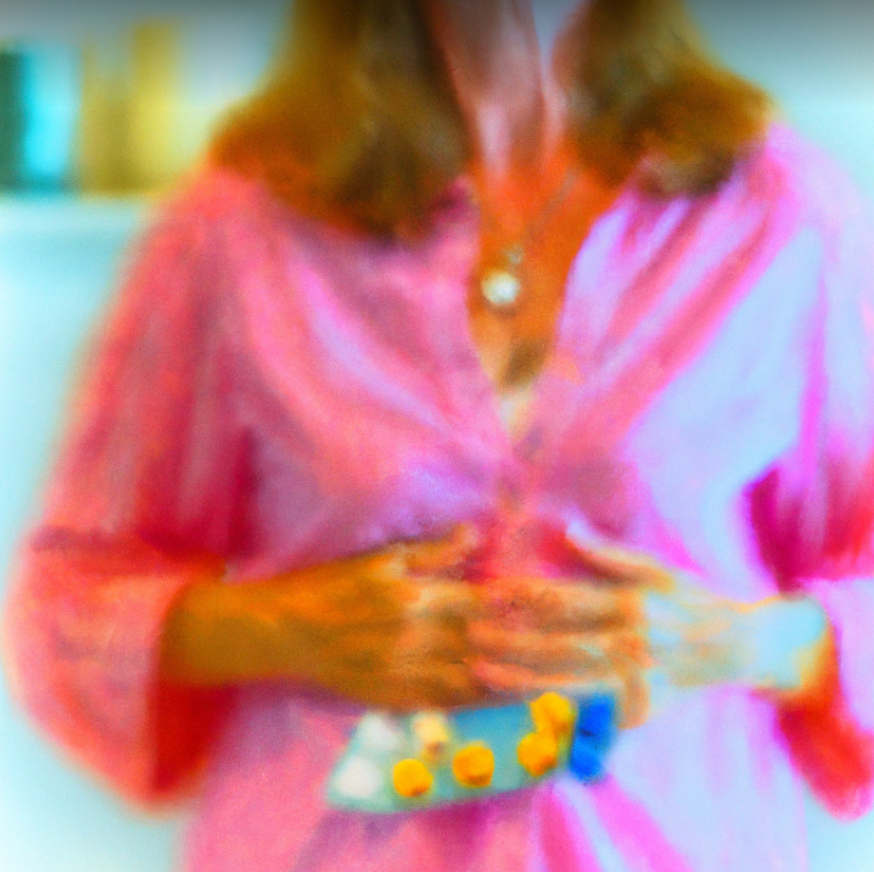
\includegraphics{./graphics/sample_2.png}} &
            \adjustbox{width=4cm,padding=5pt}{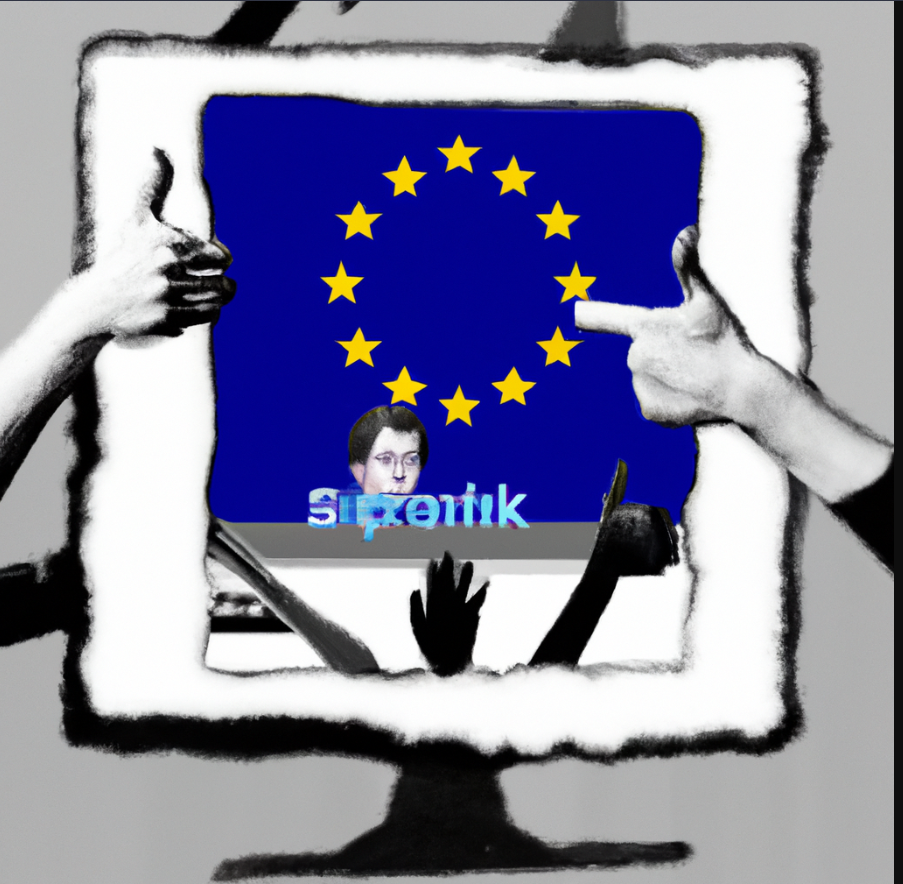
\includegraphics{./graphics/sample_3.png}} \\
            \hline
            \textbf{Referentie} & \textbf{Sample 1} & \textbf{Sample 2} & \textbf{Sample 3} \\
            \hline
            Datum & Zaterdag 20 Mei & Zondag 21 Mei & Maandag 22 Mei \\
            \hline
            Gebruikte prompt & "Eenheid voor Oekraïne" in Realistische stijl. &Women's Menopause Symptoms Relieved by Promising New Drug Style: Impressionism. & "Europese Unie geeft Facebook's Meta een recordboete" - Stijl: Surrealisme . \\
            \hline
            Inspiratie  (volgens GPT) & De prompt was gebaseerd op de kernboodschap die  eerder had gegenereerd op basis van het artikel over Charles Michel en de G7-landen die een langetermijnhulpplan en druk uitoefenden voor Oekraïne. & De kernboodschap die ik heb gegenereerd, is gebaseerd op het artikel "Nieuw medicijn tegen opvliegers op komst: ‘60 tot 70 procent van de vrouwen heeft er last van’", dat in het gegeven JSON-bestand wordt genoemd. & Deze prompt is afgeleid van de belangrijkste titel uit de JSON-gegevens die door de gebruiker zijn verstrekt, met name: "EU geeft Facebook-moederbedrijf Meta recordboete van 1,2 miljard euro". Ik heb de titel verkort tot een gepaste lengte. \\
            \hline
        \end{tabular}
        \caption{Eerste 3 gebruikte samples binnen de turingtest.}
        \label{table:samples}
    \end{table}


    \begin{table}[htbp]
    \centering
    \begin{tabular}{|p{2cm}|p{5.3cm}|p{5.3cm}|}
        \hline
        & 
        \adjustbox{width=5cm,padding=5pt}{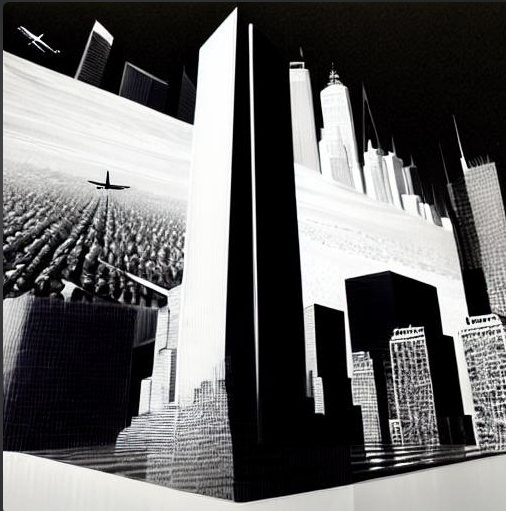
\includegraphics{./graphics/sample_4.png}} &
        \adjustbox{width=5cm,padding=5pt}{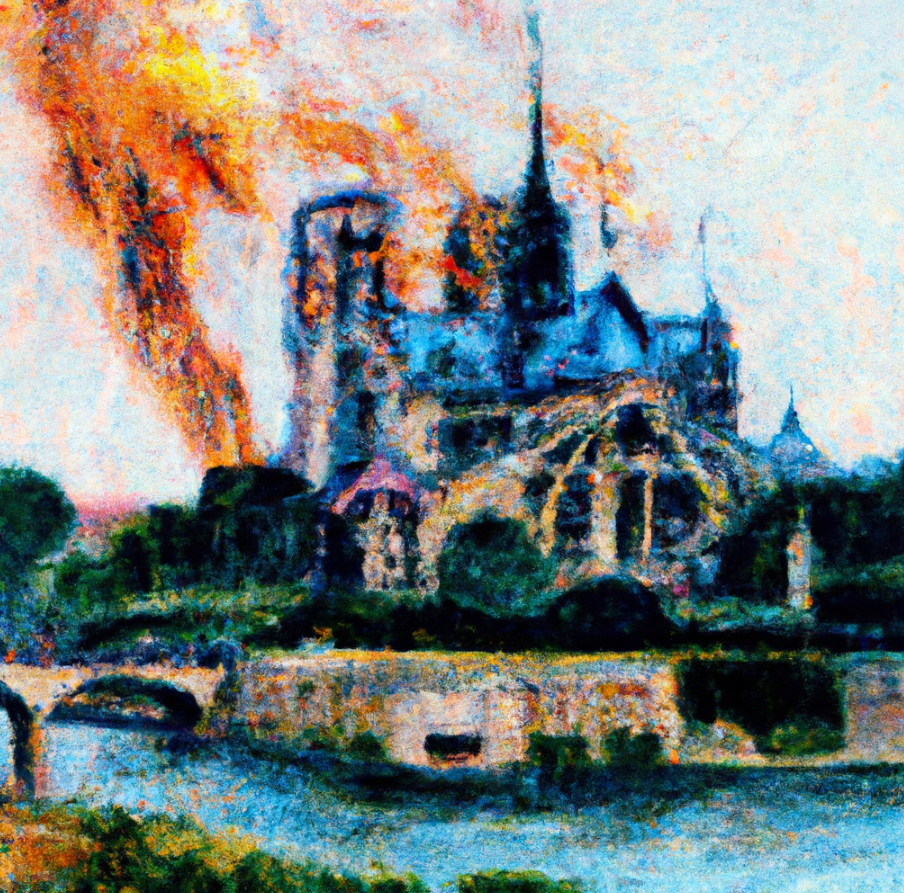
\includegraphics{./graphics/sample_5.png}} \\
        \hline
        \textbf{Referentie} &  \textbf{Sample 4} & \textbf{Sample 5} \\
        \hline
        Gebeurtenis &Terroristische aanslagen op het World Trade Center (11-9-2001) &  Brand in de Notre-Dame-kathedraal in Parijs.(15-4-2019) \\
        \hline
        Gebruikte prompt & 'Het verlies van onschuld en levens. Herdenk 9/11 met een modern kunstwerk in zwart-wit." - Stijl: Abstract-expressionisme.. & Symboliseer herstelkracht Notre-Dame na verwoestend vuur met hoopvolle, realistische elementen. Stijl: impressionisme. - Monet \\
        \hline
        Inspiratie (volgens GPT) & Mijn prompt was geen directe afspiegeling van een specifiek artikel of artikel titels. Het was bedoeld als een algemene prompt die de kernboodschap van de gebeurtenissen op 9/11 weergeeft in combinatie met de moderne kunststijl van het abstract-expressionisme in zwart-wit.& Ik heb me gebaseerd op de kernzin "Maak een kunstwerk dat de kracht en schoonheid van de Notre-Dame voorstelt, in combinatie met het tragische vuur dat de wereld heeft geschokt en de kracht van de menselijke spirit om te herstellen en te herbouwen." uit de vorige vraag. Voor deze prompt heb ik deze kernzin in een korte, bondige omschrijving omgezet die de artistieke stijl aangeeft \\
        \hline
    \end{tabular}
    \caption{Belangrijke gebeurtenissen gebruikt binnen de turingtest.}
    \label{table:events_samples}
\end{table}
\pagebreak
\section{Resultaat}
\label{section:result}
Binnen deze sectie zullen we kort de resultaten van de turingtest bespreken. \\

Bij de eerste 3 samples waarbij we op de huidige dag het nieuws hebben gescrapet, merken we op dat verschillende persona de schilderijen anders interpreteren. Dit kan te maken hebben met individuele smaak, persoonlijke achtergrond of andere factoren die van invloed zijn op hoe iemand kunstwerken waarneemt. Wat interessant is, is dat we hebben vastgesteld dat het al dan niet bekijken van het nieuws geen significante rol speelt bij de interpretatie van het schilderij. Dit suggereert dat de kunstwerken op zichzelf staan en geen specifieke voorkennis vereisen om begrepen te worden. \\

Daarnaast hebben we 2 samples gebruikt waarbij we gegevens hebben gescrapet van een specifieke dag in het verleden. Hierbij viel op dat de meeste personen de boodschap van deze kunstwerken konden afleiden. Dit duidt erop dat AI erin is geslaagd om de gewenste emotie of betekenis over te brengen op basis van belangrijke data uit het verleden.  \\

Hoewel er variatie was in de interpretaties van de kunstwerken, kunnen we concluderen dat de turingtest over het algemeen geslaagd is. Het vermogen van de kunstwerken om emoties op te roepen, betekenissen over te brengen en reacties uit te lokken, toont aan dat ze een waardevolle artistieke waarde hebben. Bovendien benadrukt het resultaat van de turingtest de veelzijdigheid en subjectiviteit van kunst. \\

De gedetailleerde resultaten van de turingtest zijn beschikbaar in bijlage punt \ref{bijlage:result_turingtest}. Daar kun je meer informatie vinden over de individuele interpretaties en feedback van de deelnemers.

 
\section{Meer uitleg}
Het resultaat verkregen van GPT en DALL-E is gebaseerd op patronen en informatie die het model heeft geleerd uit de gegevens waarop het is getraind. Hoewel deze modellen goede prestaties kunnen leveren, zijn er enkele beperkingen waardoor hun output niet altijd 100\% overeenkomt met de realiteit. \\

Ten eerste kan GPT soms de context of intentie van de invoer verkeerd begrijpen of verkeerd interpreteren. Dit kan leiden tot onjuiste of ongepaste antwoorden. Het model kan gevoelig zijn voor subtiele veranderingen in de formulering van de vraag en kan daardoor onverwachte resultaten produceren. \\

Ten tweede kan DALL-E, als een generatief model voor beeldcreatie, soms afbeeldingen genereren die niet volledig relevant zijn voor het huidige nieuws of specifieke vereisten. Hoewel het model in staat is om nieuwe, unieke afbeeldingen te maken op basis van de gegeven prompt, is het niet altijd in staat om contextuele nuances of specifieke details van de gewenste afbeelding te begrijpen. \\

We kunnen besluiten uit de werking van de applicatie dat doordat er nooit eenzelfde uitkomst is en deze uitkomst kan variëren in relevantie tot het nieuws, dat er steeds menselijke controle moet zijn op de foto vooraleer deze kan gebruikt worden binnen bijvoorbeeld een krant die dagelijks een kunstwerk genereert op basis van de artikels die hierin voorkomen. 

%%=============================================================================
%% Conclusie
%%=============================================================================

\chapter{Conclusie}%
\label{ch:conclusie}
In dit onderzoek werd een antwoord gegeven op de hoofdonderzoeksvraag en deelvragen. En lichten we kort toe over mogelijke toekomstige onderzoeksmogelijkheden. 

We beginnen met een antwoord te bieden op de deelvragen omdat deze een betere context en inzicht zullen geven voor de onderzoeksvraag. 

\section{\IfLanguageName{dutch}{Deelvraag: In welke mate kan AI effectief de essentie van een nieuwsverhaal vastleggen en vertalen naar visuele kunst?}{Sub-question: To what extent can AI effectively capture the essence of a news story and translate it into visual art?}}%

In mijn mening en wat blijkt uit de turingtest kan AI in zekere mate effectief de essentie van een nieuwsverhaal vastleggen en vertalen naar visuele kunst. Het belangrijkste aspect is het gebruik van de juiste prompts bij GPT om de gewenste resultaten te verkrijgen. Het komt echter voor dat tijdens de conversatie GPT niet altijd in staat is om het hoogtepunt van het nieuwsverhaal weer te geven waar de kenmerken duidelijk zichtbaar zijn. Daarom is het van cruciaal belang om goede prompts te gebruiken en de conversatie met het model aan te gaan. \\

Daarnaast moet worden opgemerkt dat kunst abstract is en dat iedereen kunst anders interpreteert. In sommige gevallen kan GPT een zeer abstract kunstwerk genereren, waardoor de boodschap van het nieuwsverhaal niet direct herkenbaar is. Dit kan invloed hebben op de mate waarin AI in staat is om de essentie van het nieuwsverhaal accuraat over te brengen in visuele kunst. \\

Het is ook belangrijk om aan te vullen dat de resultaten van AI-gegenereerde kunstwerken sterk afhankelijk zijn van de trainingsgegevens en het model zelf. Het is mogelijk dat AI bepaalde nuances of complexe aspecten van een nieuwsverhaal niet volledig kan vastleggen, omdat het model alleen kan putten uit de informatie waarmee het is getraind. \\

Kortom, hoewel AI in staat is om de essentie van een nieuwsverhaal te vertalen naar visuele kunst, zijn er uitdagingen en beperkingen verbonden aan het proces. Het juist formuleren van prompts, het voeren van een dialoog met het model en het begrijpen van de abstracte aard van kunst kunnen bijdragen aan het vergroten van de effectiviteit van AI bij het vertalen van nieuwsverhalen naar visuele kunst.
    
\section{\IfLanguageName{dutch}{Deelvraag: Hoe kunnen technologieën zoals GPT en DALL-E worden toegepast in de context van kunst, communicatie en maatschappij? }{Sub-question: How can technologies such as GPT and DALL-E be applied in the context of art, communication and society?}}%

Zoals wellicht duidelijk is uit deze paper zou het in eerste instantie gebruikt kunnen worden om kunst te genereren in een krant of nieuwswebsite. Zo kun je bij elk artikel een kunstwerk laten genereren , of eventueel per thema het hoogtepunt gaan kenmerken aan de hand van een schilderij.   \\

In de context van communicatie kunnen GPT en DALL-E worden gebruikt voor het genereren van content. Bijvoorbeeld, marketing- en reclamebureaus kunnen GPT gebruiken om aantrekkelijke advertentieteksten te creëren. Journalisten kunnen GPT gebruiken om nieuwsartikelen te schrijven of samenvattingen te genereren. \\

Tenslotte kan het gebruikt worden voor het analyseren van grote hoeveelheden tekstuele en visuele gegevens om inzichten te verkrijgen over maatschappelijke problemen en trends.


\section{\IfLanguageName{dutch}{Deelvraag: Hoe kan webscraping gebruikt worden om nieuwsartikelen te kunnen scrapen?}{Sub-question: How can web scraping be used to scrape news articles?}  }%
Om webscraping effectief toe te passen, is het belangrijk om de DOM-structuur van de nieuwswebsites te analyseren. Hierbij onderzoek je de HTML-elementen, tags en klassen die de relevante informatie bevatten, zoals de titels, inhoud en auteurs van de nieuwsartikelen. Door patronen te herkennen of consistente structuren te identificeren, kun je een aanpak ontwikkelen om deze informatie te extraheren. \\

Met behulp van de gekozen tool kun je nu de webscraper gaan implementeren. Hiermee stel je HTTP-verzoeken in naar de doelwebsites, extraheer je de relevante gegevens met behulp van CSS-selectors, en sla je de geëxtraheerde informatie op in een geschikt formaat.  \\

Het is belangrijk om op te merken dat websites regelmatig hun structuur en lay-out kunnen wijzigen, wat gevolgen kan hebben voor je scraper. Daarom is het goed om je scraper op een manier te implementeren dat hij minder specifiek is, maar veralgemeend.

\section{\IfLanguageName{dutch}{Onderzoeksvraag: Is AI geavanceerd genoeg om kunstwerken te genereren waarvan de boodschap herkenbaar is uit het dagelijks nieuws?}{Research question: Is AI advanced enough to generate works of art whose message is recognizable from the daily news?}  }%
Op basis van voorgaande deelvragen kunnen we besluiten dat met de opkomst van AI-technologieën  het mogelijk is geworden om kunstwerken te genereren die gebaseerd zijn op nieuwsartikelen en/of andere tekstbronnen. \\

De kunstwerken kunnen de essentie van het nieuwsverhaal vastleggen en vertalen naar visuele vormen, maar er zijn uitdagingen en beperkingen verbonden aan dit proces. Het gebruik van de juiste prompts bij GPT en het begrijpen van de abstracte aard van kunst zijn essentiële factoren om de effectiviteit van AI te vergroten bij het vertalen van nieuwsverhalen naar visuele kunst. Bovendien kunnen technologieën zoals GPT en DALL-E breder worden toegepast in de context van kunst, communicatie en maatschappij. Ze kunnen bijvoorbeeld gebruikt worden voor het genereren van content, zoals advertentieteksten, nieuwsartikelen of andere zaken.


\section{\IfLanguageName{dutch}{Verdere onderzoeksmogelijkheden}{Further research opportunities}  }%
De resultaten van dit onderzoek hebben inzichten opgeleverd met betrekking tot de mogelijkheden en uitdagingen van AI bij het genereren van kunstwerken op basis van nieuwsverhalen. Niettemin zijn er nog verschillende interessante vragen en onderzoeksperspectieven die verder kunnen worden verkend. Zo kan er toekomstig onderzoek worden gedaan naar de mate van accuraatheid en coherentie van AI-modellen bij het overbrengen van de boodschap van nieuwsverhalen in visuele kunst. Daarnaast kan er gekeken worden naar de integratie van abstracte aspecten van kunst in AI-algoritmen om meer expressieve en interpretatieve kunstwerken te genereren.  Daarnaast kunnen ook de mogelijkheden van AI-gestuurde kunstwerken in de journalistiek en communicatie verder worden onderzocht, evenals de rol van menselijke input in dit proces.

% TODO: Trek een duidelijke conclusie, in de vorm van een antwoord op de
% onderzoeksvra(a)g(en). Wat was jouw bijdrage aan het onderzoeksdomein en
% hoe biedt dit meerwaarde aan het vakgebied/doelgroep? 
% Reflecteer kritisch over het resultaat. In Engelse teksten wordt deze sectie
% ``Discussion'' genoemd. Had je deze uitkomst verwacht? Zijn er zaken die nog
% niet duidelijk zijn?
% Heeft het onderzoek geleid tot nieuwe vragen die uitnodigen tot verder 
%onderzoek?




% Voeg hier je eigen hoofdstukken toe die de ``corpus'' van je bachelorproef
% vormen. De structuur en titels hangen af van je eigen onderzoek. Je kan bv.
% elke fase in je onderzoek in een apart hoofdstuk bespreken.

%\input{...}
%\input{...}
%...


%---------- Bijlagen -----------------------------------------------------------

\appendix
\chapter{\IfLanguageName{dutch}{Codefragmenten}{Codefragments}}%
\label{ch:code_fragments}
\section{Resultaat scraper}
\begin{listing}
    \label{bijlage:json-input}
    \begin{minted}[breaklines]{json}
        {
            "https://www.hln.be": [
            "Nederlander (37) overlijdt na ongeval met ontplofte petanquebal tijdens vrijgezellenfeest in Stavelot",
            "EXCLUSIEVE ANALYSE. “Oekraïne heeft 4 mirakels nodig”",
            "Staatssecretaris Bertrand spreekt straffe taal tegen banken: “Maar de overheid moet zelf ook het goede voorbeeld geven”",
            "“Russisch leger rekruteerde dit jaar al bijna 120.000 soldaten”",
            "Barack Obama niet meer welkom in Rusland: inreisverbod tegen voormalige president en 499 andere Amerikanen",
            "Opmars Aziatische hoornaar niet meer te stuiten in Vlaanderen: \"Kwestie van tijd voor er doden vallen”",
            "Nederlander (37) overlijdt na ongeval met ontplofte petanquebal tijdens vrijgezellenfeest in Stavelot",
            "Poetins geheime bunkercomplex onder gigantisch paleis aan Zwarte Zee onthuld: zo ziet het eruit"
            ],
            "https://www.demorgen.be": [
            "Voor de mensen achteraan in de zaal: het is absoluut zeker dat de klimaatverandering tot meer extreme weersituaties leidt",
            "Pedagoog Pedro De Bruyckere: ‘Leerlingen in Engeland en Ierland zitten ook constant op hun smartphone, en zij gingen erop vooruit’",
            "Transgender activiste Jenna Boeve: ‘Als ik in lingerie naar de Pride ga, is dat ook een vorm van protest’",
            "Waarom meer geliefden hebben (niet) altijd beter is: ‘Fantastisch om je partner te vertellen dat je verliefd bent op een ander’",
            "Jane Fonda: ‘Franse regisseur vroeg me om met hem naar bed te gaan ‘om te zien hoe mijn orgasmes waren’ voor een rol’",
            "Enorme gewicht van wolkenkrabbers brengt New York in problemen bij verwachte zeespiegelstijging",
            "Rubio wint bergrit van 74 kilometer, wapenstilstand onder favorieten",
            "Britse telecomreus vervangt 10.000 jobs door AI",
            "‘VS zetten licht op groen voor training Oekraïense piloten in westerse gevechtsvliegtuigen’",
            "Live - Oekraïne. Rusland vaardigt arrestatiebevel uit tegen aanklager Internationaal Strafhof die Poetin wil laten arresteren",
            "‘Helft leerlingen secundair onderwijs heeft moeite met lezen’",
            "Erdogan prijst ‘speciale relatie’ met Poetin: ‘Rusland en Turkije hebben elkaar nodig op alle vlakken’",
            "‘Ook aan hun kant ontploft er heel wat’: Oekraïne lijkt te dralen met zijn tegenoffensief",
            "‘VS zetten licht op groen voor training Oekraïense piloten in westerse gevechtsvliegtuigen’"
            ]
        }
        
    \end{minted}
    \captionof{figure}{De gescrapete json-data op vrijdag 19 mei 20:07}
\end{listing}
\pagebreak


\section{Implementatie Scraper op specifieke dag}
\label{bijlage:changes_scraper}
\subsection{Aanpassing gesprek GPT}
Omdat we nu op een specifieke dag scrapen, kunnen we dit ook meegeven aan GPT. Verder doen we kleine aanpassingen aan de conversatie voor betere resultaten. Hieronder vindt je de nieuwe implementatie van GPT. 
\begin{pythoncode}{../../../workspace/paper/gpt2.0.py}
\end{pythoncode}

\subsection{Implementatie scraper}
Om te kunnen scrapen op een specifieke dag, en niet uren willen wachten tot de scraper alle artikels van een website heeft overlopen, scrapen we nu het archief van de Standaard. In volgende code-fragment vind je de geïmplementeerde scraper. 
\begin{pythoncode}{../../../workspace/paper/StandaardScraper.py}
    Merk op de scraper gebruikt nu HTMLSession() om de DOM-structuur te parsen, dit is omdat met bs4 het niet mogelijk was. 
\end{pythoncode}

\subsection{Aanpassingen \_\_main\_\_.py}
Uiteraard moeten we nu ook de \_\_main\_\_.py aanpassen zodat hij deze wijzigingen uitvoerd. In volgende code-fragment zie je de wijzigingen. 

\begin{pythoncode}{../../../workspace/paper/newMain.py}

\end{pythoncode}




\chapter{\IfLanguageName{dutch}{Resultaten: Turingtest}{Results: Turingtest}}%
In dit onderzoek is een Turingtest uitgevoerd om de prestaties van het AI-model te evalueren. De uitleg van de Turingtest zijn te vinden in sectie \ref{sec:turingtest} van het evaluatieproces. Hieronder vindt je de resultaten van de turingtest opgelijst per persona. 
\section{Resultaten Turingtest}
\label{bijlage:result_turingtest}
\subsection{Persona: Ronan}
Ronan is een creatieve ICT-student die graag game development wil studeren. Hij is een getalenteerde tekenaar, maar hij volgt geen nieuws.
\subsubsection{Sample 1}
Bij het bekijken van het schilderij merkt Ronan op: "Dat in het midden is niet echt duidelijk, maar het lijkt erop dat er verschillende landen iets willen doen in Oekraïne." \\

Ronan lijkt de kernboodschap van dit schilderij matig te hebben begrepen. Hij heeft opgemerkt dat er verschillende landen betrokken zijn bij een kwestie in Oekraïne. Hoewel hij niet specifiek weet welk artikel hieraan ten grondslag ligt, heeft hij de basis toch begrepen.  \\

Ronan vertelde me dat als de vlaggen die centraal worden afgebeeld een betekenis hadden, indien hij wist waarvoor de vlaggen stonden kon hij waarschijnlijk de kernboodschap hieruit afleiden. 

\subsubsection{Sample 2}
Bij het analyseren van dit schilderij geeft Ronan zijn interpretatie: "Iets met medicatie, een nieuw medicijn en/of anticonceptiemiddel? Wat de vrouw in haar hand houdt, kan misschien een nieuw geneesmiddel zijn dat op de markt is gelanceerd." \\

Ronan heeft de boodschap van dit schilderij opgepikt en vermoedt dat het gaat over medicatie. Hij suggereert dat er mogelijk een nieuw medicijn of anticonceptiemiddel is ontwikkeld, en de vrouw in het schilderij houdt misschien het nieuwe geneesmiddel vast. Hoewel hij niet precies weet welk artikel hieraan gerelateerd is, heeft hij een algemeen begrip van het onderwerp. \\

\subsubsection{Sample 3}
"Ik zie iets met Europa, een duim omhoog wat duidt op goedkeuring. Het lijkt op een computerscherm, dus misschien heeft het iets te maken met een website. Ik denk dat het Europees Parlement een nieuwe wet heeft goedgekeurd die te maken heeft met regels op het internet." \\

Ronan heeft de boodschap niet kunnen achterhalen. Hij heeft wel opgemerkt dat de EU duidelijk aanwezig is in het schilderij, maar hij herkende de duimpjes niet als de iconische "likes" op Facebook. Na het tonen van het artikel zei Ronan dat het mogelijk was geweest om dit te herkennen, maar dat abstractie correct geïnterpreteerd moet kunnen worden.

\subsubsection{Sample 4}
In Sample 4 heeft Ronan zonder enige twijfel verteld dat dit de aanslagen op de bekende Twin Towers weerspiegeld. Zijn directe herkenning van deze gebeurtenis toont aan dat het schilderij een duidelijk visueel verband had met een historisch moment dat wereldwijd bekend is. \\

De gebeurtenis van deze schilderij werd meteen achterhaald.

\subsubsection{Sample 5}
In Sample 5 twijfelde Ronan even voordat hij bevestigde dat het schilderij de Notre-Dame toonde tijdens de verwoestende brand. Hoewel er een kort moment van aarzeling was, slaagde Ronan erin om de gebeurtenis correct te identificeren. Dit laat zien dat het schilderij voldoende visuele aanwijzingen bevatte om de specifieke gebeurtenis te herkennen, zelfs als er enige interpretatie of herinnering nodig was. \\

Deze sample bewijst dat het mogelijk is om betekenisvolle gebeurtenissen via kunstwerken te onthullen. 


\subsection{Persona: Arthur}
Arthur is een laatstejaarsstudent Informatica met een matige kennis van kunst. Hoewel hij zelf niet actief betrokken is bij het creëren van kunst, heeft hij een goed begrip van het onderwerp. Arthur volgt het nieuws niet. 

\subsubsection{Sample 1}
Arthur merkte het volgende op: ``Dit gaat gegarandeerd over Oekraïne. Het lijkt erop aan de hand van de vlag dat een groep landen samenwerken binnen Oekraïne voor één bepaald doel.'' \\

We besluiten dat arthur de boodschap van dit schilderij goed begrepen heeft en concludeert dat het gaat over samenwerking tussen landen in Oekraïne. Hoewel hij niet specifiek weet welk artikel hieraan gerelateerd is, heeft hij de essentie begrepen. 

\subsubsection{Sample 2}
Arthur merkte het volgende op: "Op het eerste zicht lijkt het alsof een vrouw in dit schilderij lijdt. Ik zie ook medicatie haar liggen. Zou dit kunnen gaan over de nieuwe medicatie voor vrouwen die in hun menopauze zitten?" \\

Arthur heeft de boodschap van dit schilderij opgepikt en vermoedt dat het te maken heeft met het lijden van vrouwen. Hij maakt de associatie met medicatie en suggereert dat het mogelijk gaat over nieuwe medicatie voor vrouwen in hun menopauze. 

\subsubsection{Sample 3}
Arthur had de volgende interpretatie: ``Iets met europese unie, iets dat goedgekeurd moet worden of al is gebeurd?'' \\

Arthur heeft de boodschap van dit schilderij niet specifiek kunnen achterhalen, maar hij herkent de aanwezigheid van de Europese Unie. Hij vermoedt dat het schilderij mogelijk te maken heeft met goedkeuring van iets, ofwel iets dat nog moet gebeuren of al heeft plaatsgevonden. Doordat hij geen specifieke details of context kan geven, heeft hij de boodschap niet kunnen achterhalen. 

\subsubsection{Sample 4}
Bij het bekijken van het schilderij moest Arthur toch even nadenken. Na het opmerken van het vliegtuig, maakte hij de gok dat het verband hield met de gebeurtenis van 9/11. Het bleek een goede gok te zijn, aangezien zijn interpretatie juist was.

\subsubsection{Sample 5}
Bij het aanschouwen van het schilderij kon Arthur niet direct de specifieke gebeurtenis identificeren, en beschreef hij het simpelweg als "een brandende kerk aan het water". Pas nadat ik hem vertelde dat het de afbeelding van de Notre-Dame in Parijs betrof, vond hij het schilderij zeer duidelijk. Het bleek dat hij gewoon niet aan die specifieke gebeurtenis had gedacht, maar de boodschap van het schilderij kwam alsnog goed bij hem over.

\subsection{Persona: Arjan}
Arjan is geboren in Turkije en opgegroeid in Nederland. In zijn jongere jaren heeft hij zich veel beziggehouden met het ontwerpen van logo's en banners voor profielen, wat zijn vaardigheden op het gebied van grafisch ontwerp versterkt. Dit maakt hem een interessante testpersona voor de turingtest, aangezien zijn ervaring en kennis een waardevolle troef kunnen zijn. Arjan volgt enkel de hoogtepunten van het nieuws.

\subsubsection{Sample 1}
``Ik kan dit artikel niet helemaal plaatsen. Hoewel het over Oekraïne gaat, kan ik de boodschap er niet uit halen. Als ik zou moeten gokken, zou ik zeggen dat er meerdere landen bij betrokken zijn vanwege de aanwezigheid van vlaggen. Maar ik kan de precieze boodschap niet achterhalen.'' \\

Net als de vorige persona kan Arjan ook concluderen dat het artikel over Oekraïne gaat en dat andere landen mogelijk betrokken zijn. De boodschap blijft echter onduidelijk.

\subsubsection{Sample 2}
Arjan vermoedde dat dit kunstwerk ging over een vrouw die verslaafd is aan medicatie. Echter, toen ik hem vertelde dat het eigenlijk ging over een nieuwe medicatie, kon hij meteen zeggen dat het specifiek ging over medicatie voor de menopauze. \\

De oorspronkelijke boodschap werd dus verkeerd geïnterpreteerd door Arjan. Echter, met een hint kon hij wel de juiste boodschap interpreteren.

\subsubsection{Sample 3}
"Europese Unie, televisie, duimen. Heeft dit misschien iets te maken met Facebook? Gaat dit over de boete die de Europese Unie heeft opgelegd aan Meta?" \\

Arjan heeft de mogelijke connectie gelegd tussen de Europese Unie, televisie en duimen, en vermoedt dat het mogelijk verband houdt met Facebook. Hij suggereert dat het specifiek zou kunnen gaan over de boete die de Europese Unie heeft opgelegd aan Meta. \\

Arjan heeft successvol de boodschap hieruit gehaald en ook de correcte artikel hieraan gelinkt. 

\subsubsection{Sample 4}
Bij het bekijken van de schilderij, herkende Arjan onmiddellijk dat de Twin Towers het centrale onderwerp waren. Aan de hand van de de vliegtuigen op het schilderij legt Arjan direct het verband met de gebeurtenissen van 9/11. \\

Zijn interpretatie was correct en hij twijfelde niet over de boodschap die het schilderij overbracht.

\subsubsection{Sample 5}
Arjan had geen enkel probleem met hier de betekenis eruit te halen. Hij kon duidelijk zeggen dat dit over de Notre-Dame gaat in Parijs die enkele jaren geleden in brand stond. 

\subsection{Persona: Lucas}
Lucas is een gepassioneerde software engineer die in zijn vrije tijd graag muziek draait. Hoewel hij geen specifieke artistieke achtergrond heeft, is hij wel creatief in zijn vakgebied. Lucas volgt echter het nieuws niet.
\subsubsection{Sample 1}
Bij het bekijken van het schilderij herkende Lucas een gevoel van patriotisme en merkte hij op dat de rode lijn in Oekraïne mogelijk een splitsing of een grens vertegenwoordigde. Hij kon echter geen verband leggen tussen de vlaggen en meerdere landen. Met andere woorden, Lucas kon de exacte boodschap van dit schilderij niet achterhalen.
\subsubsection{Sample 2}
Het wazige beeld en de afbeelding van medicatie deden Lucas denken aan een verslaving. Toen ik hem vertelde dat het schilderij eigenlijk ging over een nieuw medicijn voor vrouwen, kon Lucas de link leggen en begrijpen waar het over ging.
\subsubsection{Sample 3}
Lucas interpreteerde dit schilderij als iets waarover gestemd moest worden. De mensen die hun duim omhoog staken, suggereerden dat er een nieuwe regel of wet werd beoordeeld. Nadat ik hem vertelde dat de duimen eigenlijk het Facebook-symbool waren, kon hij de link leggen, maar slaagde hij er nog steeds niet in om de exacte boodschap eruit te halen.
\subsubsection{Sample 4}
De boodschap van deze sample kwam duidelijk over bij Lucas. Hoewel hij aanvankelijk een kleine twijfel had, kon hij uiteindelijk bevestigen dat het schilderij betrekking had op de gebeurtenissen van 9/11. Zijn interpretatie was helder en de boodschap kwam zeker goed over.

\subsubsection{Sample 5}
Lucas herkende direct dat het schilderij de Notre-Dame in Parijs afbeeldde. Hij verklaarde: "Omdat deze gebeurtenis nog vers in het geheugen zit, kon ik het waarschijnlijk gemakkelijk herkennen."

\subsection{Persona: Gustas}
Gustas is een Litouwse man met een sterke interesse in automatisering. Hij heeft zijn studies stopgezet om zijn eigen bedrijf op te richten. Gustas heeft gedurende 4 jaar gestudeerd aan een kunstschool. Vanwege zijn nationaliteit en achtergrond in de kunst lijkt deze persona zeer interessant voor de turingtest. Het feit dat Gustas het nieuws niet volgt, voegt een interessant perspectief toe aan zijn beoordeling van de kunstwerken.

\subsubsection{Sample 1}
Bij het eerste voorbeeld merkte Gustas de volgende boodschap op: "Ik denk dat het nieuws gaat over Oekraïne die een deel van het land terugneemt?" Helaas was dit niet de juiste boodschap. Gustas gaf aan dat de rode lijn in het kunstwerk deed vermoeden dat het een bezet gebied van Rusland was. \\

Na de vraag te stellen: "Zou je de boodschap in het schilderij herkennen nadat je het artikel hebt gelezen?" reageerde Gustas met: "Voor mij geeft niets aan dat het over een G7-bijeenkomst gaat." \\

De juiste boodschap werd niet uit dit voorbeeld gehaald.

\subsubsection{Sample 2}
Bij het tweede kunstwerk merkte Gustas op dat het zeker over gezondheidsproblemen ging. Hij vroeg zich af of er een nieuw medicijn was gekomen voor tijdens de zwangerschap. \\

Hoewel de boodschap gedeeltelijk juist was, was het specifieke medicijn eigenlijk bedoeld voor de menopauze, niet voor tijdens de zwangerschap. \\

Gustas bevestigde dat hij dit wel degelijk in het kunstwerk zag, maar erkende dat het zeer moeilijk is om de menopauze uit te beelden binnen een schilderij.

\subsubsection{Sample 3}
Het derde kunstwerk werd tot nu toe het best geïnterpreteerd door Gustas. Hij kon afleiden dat de Europese Unie op de een of andere manier verband hield met Facebook, maar wist niet precies hoe. Hij vermoedde dat er een nieuwe regel was opgelegd aan Facebook. \\

Gustas zat er heel dichtbij, maar net niet helemaal. Nadat hij het artikel had gezien, vroeg ik hem of hij nu de boodschap uit het schilderij kon halen. \\

Hij was hier niet zeker van omdat er niets was dat aanduidde dat het met geld te maken had.

\subsubsection{Sample 4}
In eerste instantie kon Gustas de gebeurtenis van 9/11 niet direct herkennen in het schilderij. Na enkele ogenblikken, werd het hem uiteindelijk duidelijk en kon hij de boodschap achter het kunstwerk ontcijferen.

\subsubsection{Sample 5}
Bij het laatste schilderij was de boodschap voor Gustas duidelijk, alhoewel hij aanvankelijk een vergissing maakte. Hij dacht dat het ging over een kerk die in brand was gestoken in Spanje, maar even later corrigeerde hij zichzelf en gaf toe dat hij de Notre-Dame in Frankrijk bedoelde. Ondanks de initiële verwarring, begreep Gustas uiteindelijk de boodschap van het schilderij. \\

Het is duidelijk dat de boodschap van beide schilderijen wel degelijk succesvol overkwam bij Gustas.

\subsection{Persona: Shauny}
Shauny is een laatstejaarsstudente Journalistiek aan de Arteveldehogeschool met een grote interesse in politiek. Shauny volgt bijna dagelijks het nieuws en heeft enkele maanden bij een nieuwszender gewerkt als journaliste. Ze lijkt me een perfecte persona voor deze turingtest.

\subsubsection{Sample 1}
Shauny merkte op: "Gaat dit over iets met Bakhmut? Het is moeilijk om te zeggen, ik heb geen idee wat die vlaggen of het wapenschild betekenen. Is het mogelijk een groep landen die samenkomen om iets te doen?" \\

Shauny had grotendeels de kernboodschap begrepen uit dit artikel maar kon niet de link leggen met de G7-bijeenkomst.  \\

Na het tonen van de artikel, kon Shauny nu wel de betekenis hieruit halen. 
Shauny had grotendeels de essentiële boodschap begrepen uit dit artikel, maar kon de link met de G7-bijeenkomst niet leggen. \\

Nadat het artikel was getoond, kon Shauny nu wel de betekenis ervan afleiden.
"Als ik dit artikel had gezien of gelezen, dan zou ik waarschijnlijk aan zoiets hebben gedacht."

\subsubsection{Sample 2}
Shauny kon meteen afleiden uit het schilderij dat het ging over een vrouw die last had van haar buik. Ze dacht dat er mogelijk een probleem was met anticonceptiepillen. Echter, ze kon niet precies afleiden dat het eigenlijk ging om nieuwe medicatie voor de menopauze.\\

Na het tonen van het artikel kon Shauny echter wel duidelijk de betekenis ervan afleiden.

\subsubsection{Sample 3}
Bij deze sample dacht Shauny dat er gestemd werd over Griekenland in verband met een bepaalde nieuwe regel. Echter, nadat haar werd verteld dat de duimpjes symbool stonden voor Facebook, dacht ze dat er nieuwe regels voor Facebook werden opgesteld. \\

Toen Shauny het artikel te horen kreeg, vertelde ze me dat ze waarschijnlijk de boodschap hieruit niet kon afleiden. Ze gaf aan dat er enkele elementen ontbraken die aangaven dat het om een boete ging.

\subsubsection{Sample 4}
Shauny herkende onmiddellijk de associatie met de gebeurtenis van 9/11 bij het bekijken van dit schilderij. Haar interpretatie was correct en ze begreep direct de boodschap van de sample.

\subsubsection{Sample 5}
Net zoals bij de vorige sample kon Shauny vrijwel direct de boodschap uit dit schilderij halen. Haar vermogen om de betekenis ervan snel te begrijpen, toont aan dat de boodschap effectief werd overgebracht en begrepen werd door Shauny.

\subsection{Persona: Filip}
Filip is een busschauffeur met een passie voor schilderen en het maken van collages. Hij is een zeer creatieve persoon vol inspiratie en probeert dagelijks het nieuws te volgen.

\subsubsection{Sample 1}
Bij het tonen van het eerste kunstwerk dacht Filip dat het ging over een bijeenkomst in Oekraïne, waar politici van verschillende landen samenkwamen met de president van Oekraïne om een plan te bedenken met betrekking tot Rusland. \\

Hoewel de boodschap grotendeels begrepen werd, kon de specifieke link naar het juiste artikel niet worden gelegd.

\subsubsection{Sample 2}
Het volgende schilderij werd iets moeilijker geïnterpreteerd door Filip. Hij meende dat de vrouw leed onder verkeerde medicatie en vermoedde dat het ging over situaties waarin artsen vaak verkeerde medicatie voorschrijven aan patiënten. \\

Na het vertellen dat het eigenlijk ging over nieuwe medicatie voor vrouwen tijdens de menopauze, kon hij deze boodschap wel duidelijk herkennen. Het kunstwerk kon echter met meerdere zaken in verband worden gebracht vertelde Filip.

\subsubsection{Sample 3}
Bij het 3e kunstwerk zag Filip verschillende elementen naar voren komen, zoals een televisie, de Europese Unie, het vind-ik-leuk-symbool en vragen. \\

Filip interpreteerde de boodschap van dit schilderij als volgt: "De Europese Unie heeft nieuwe regels opgelegd, waarbij mensen in het parlement het eens waren of vragen hadden. Maar de inwoners en televisiekijkers hadden gemengde gevoelens hierover." \\

Ondanks de inspiratie en creativiteit van Filip werd de boodschap volledig anders geïnterpreteerd. Nadat het artikel aan Filip werd voorgelezen, gaf hij aan dat deze boodschap te abstract was om eruit te halen. Misschien als hij het "vind-ik-leuk"-symbool had geïnterpreteerd als Facebook, zou het beter gelukt zijn.

\subsubsection{Sample 4}
Filip kon onmiddellijk de boodschap achterhalen bij de sample die verwees naar de 9/11-gebeurtenis. Voor hem was deze sample zeer duidelijk en begrijpelijk.

\subsubsection{Sample 5}
Na even twijfel wist Filip mij te vertellen dat het schilderij betrekking had op de brandende kerk in Parijs, de Notre-Dame. Ook bij deze sample slaagde Filip erin de boodschap en betekenis uit het schilderij te halen.


\subsection{Persona: Marta}
Marta is een kinderjuffrouw die geen artistieke bezigheden heeft en zichzelf niet als creatief beschouwt. Ze volgt echter dagelijks het nieuws.

\subsubsection{Sample 1}
Marta interpreteert het volgende: "Dit heeft duidelijk iets met Oekraïne te maken, maar ik weet niet precies wat. De verschillende vlaggen die ik niet herken, suggereren mogelijk de betrokkenheid van verschillende landen." \\

Marta kon het artikel niet direct aan dit kunstwerk linken, maar begreep wel de kernboodschap ervan. Toen ik Marta vroeg of ze het artikel herkende, vertelde ze me dat Oekraïne dagelijks in het nieuws komt en het moeilijk is om een specifiek artikel daaraan te koppelen, vooral als het kunstwerk algemeen is, naar mijn mening.

\subsubsection{Sample 2}
"Gaat dit over een nieuw medicijn tijdens de menopauze?" merkte Marta op. \\

Marta kon direct het artikel hiermee in verband brengen en de boodschap begrijpen.

\subsubsection{Sample 3}
"Hmm, dit is moeilijk. Het heeft iets te maken met de Europese Unie en verschillende meningen worden eraan gekoppeld. Misschien gaat het over een nieuwe regel die is opgelegd en waar mensen uiteenlopende standpunten over hebben? Nee, ik kan het niet echt begrijpen", zei Marta. \\

Nadat ik vertelde dat het artikel gaat over een recordboete die aan Facebook is opgelegd wegens schending van privacyregels, kon Marta het er niet in herkennen. Het onderwerp is te abstract voor haar.

\subsubsection{Sample 4}
Direct na het bekijken van het schilderij kon Marta met zekerheid vaststellen dat het de WTC-torens in Amerika betrof. Ze legde de associatie met 9/11 door het aanwezige vliegtuig in de buurt van de torens.

\subsubsection{Sample 5}
Bij haar eerste indruk dacht Marta dat het een afbeelding was van een brandende kerk. Ze kon niet onmiddellijk identificeren dat het specifiek de Notre-Dame betrof. Na een hint kon ze echter wel de juiste connectie maken en begreep ze dat het schilderij inderdaad verwijst naar de Notre-Dame. Ondanks de initiële verwarring slaagde Marta er uiteindelijk in om de juiste boodschap van het schilderij te begrijpen.

\chapter{\IfLanguageName{dutch}{Onderzoeksvoorstel}{Research proposal}}%
Het onderwerp van deze bachelorproef is gebaseerd op een onderzoeksvoorstel dat vooraf werd beoordeeld door de promotor. Dat voorstel is opgenomen in deze bijlage.
%---------- Inleiding ---------------------------------------------------------

\section{Introductie}%
\label{sec:introductie}
\noindent
Traditionele nieuwsbronnen streven al geruime tijd naar objectiviteit en feitelijkheid, om informatie vanuit eenzelfde perspectief en met een vergelijkbare boodschap over te brengen. Door het hoogtepunt van de dag te abstraheren tot een uniek AI-gegenereerd kunstwerk, kan er worden geëxperimenteerd met de grenzen van de menselijke perceptie en kunst. \\
\noindent
Mijn toegepaste onderzoek richt zich op het ontwikkelen van een applicatie die kunstwerken genereert op basis van het dagelijkse hoogtepunt, waarvoor gegevens zullen worden verzameld door het 'scrapen' van nieuwswebsites en socialmediaplatformen.
Deze zal een kunstwerk genereren met behulp van één of meerdere deep learning modellen. \\
\noindent
Het doel is om te onderzoeken of AI kunstwerken kan genereren die een boodschap van het dagelijks nieuws kan overbrengen. Dit zal gebeuren met behulp van een turing test die zal bevestigen of het kunstwerk al dan niet enige emotie of boodschap overbrengt met enige relevantie tot het nieuws dat die dag gebeurd.\\
\noindent
Dit onderzoek kan interessante inzichten opleveren in de relatie tussen kunst, technologie en de samenleving.

%---------- Stand van zaken ---------------------------------------------------

\section{Literatuurstudie}%
\subsection{Wat is webscraping?} 
\noindent
Webscraping is een term die gebruikt wordt voor het extraheren van inhoud van websites om het te importeren in lokale opslag zoals een database of CSV bestand.  \autocite{Salem2020} \\
\noindent
Websites kunnen ervoor kiezen om een \emph{robots.txt} (\ref{fig:robotstxt}) in de root van hun filesystem te plaatsen. Binnen deze tekstfile kunnen ze beschrijven welke routes gescraped mogen worden. \autocite{GoogleDocs} \\
\begin{center}
    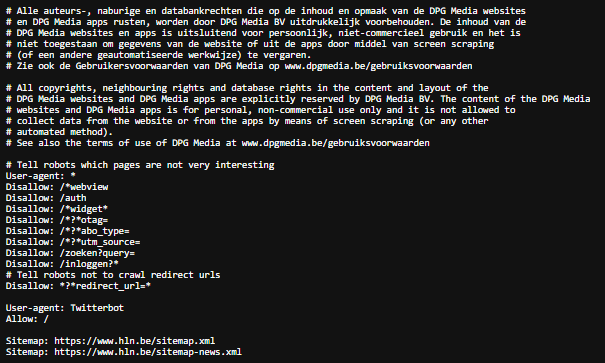
\includegraphics[width = 3in]{robotstxt_hln}
    \captionof{figure}{voorbeeld: www.hln.be/robots.txt}
    \label{fig:robotstxt}
\end{center}

\subsection{Wat is DALL-E (2)?}

\noindent
DALL-E is een AI software ontwikkeld door openAI dat beelden creëert uit tekstuele beschrijvingen, ook wel \emph{prompts} genoemd. Het gebruikt een versie met 12 miljard parameters van het GPT-3 Transformer-model om natuurlijke taalinvoer te interpreteren en overeenkomstige beelden te genereren. In april 2022 heeft OpenAI DALL-E 2 gelanceerd, ontwikkeld om meer realistische foto's met hogere resolutie te kunnen genereren. \\
 \autocite{DallEWikipediaNL}  \autocite{DallEWikipediaEN}\\

\noindent
DALL-E 2 is bovendien getrained met behulp van 650 milioen tekstinputs gescraped van het internet. \autocite{Borji2022} \\

\noindent
DALL-E 2 is niet open source maar kun je gebruiken aan de hand van de openAI API.  \\
\subsection{Wat is Stable Diffusion?}
\noindent
Stable Diffusion is een deep learning, tekst-naar-beeld model uitgebracht in 2022. In tegenstelling tot DALL-E (2) is Stable Diffusion getrained aan de hand van een diepe generatieve neurale netwerk.
\autocite{StableDifWikipediaEN}

Stable Diffusion is open source en kun je lokaal draaien op een computer met een GPU.



%---------- Methodologie ------------------------------------------------------
\section{Methodologie}%
\label{sec:methodologie}
\noindent
\textbf{Inleiding} \\
Het toegepaste onderzoek start op 2 maart 2023 en eindigt voor 28 mei 2023.

\noindent
\textbf{Fase 1: Realiseren van een scraper} \\
Om de data te bekomen van de verschillende soorten websites of social-media platformen zal er een web scraper worden gemaakt. Deze scraper zal ontwikkeld worden in python met behulp van een externe library \emph{BeautifulSoup}.

\noindent
\textbf{Fase 2: Data verwerken en analyseren} \\
Tijdens de tweede fase zullen we onderzoeken op welke manier we de bekomen data uit voorgaande fase kunnen analyseren en sorteren. \\ \\
\noindent
Het zal belangrijk zijn om rekening te houden met de volgende vragen: 
\begin{itemize}
    \item Wat zijn de te extraheren kernzaken?
    \item Wat is het sentiment van de dag? 
    \item Welke topic komt het vaakst voor?
    \item Op basis van welke gegevens kunnen we de artikels sorteren? 
\end{itemize}

\noindent
Nadat er een gepaste methode wordt gevonden om dit te realiseren, zal deze ook geïmplementeerd worden. Op deze manier kunnen we steeds het belangrijkste artikel van de dag eruit halen. \\

\noindent
\textbf{Fase 3: Kunstwerk genereren} \\
Nu dat we weten uit de vorige fase wat het hoogtepunt van de dag was. Kunnen we hierop een kunstwerk laten genereren. \\
Hiervoor zal er gebruik gemaakt worden van een of meerdere deep learning modellen DALL-E 2 en/of Stable Diffusion die de kerntekst van een artikel zal omvormen tot een foto. \\

\noindent
\textbf{Fase 4: Turing test} \\ 
Tijdens de laatste fase van dit onderzoek willen we bepalen of de AI-gegenereerde kunstwerken van DALL-E 2 en/of Stable Diffusion herkenbeer zijn uit het dagelijks nieuws. We zullen hiervoor een Turing test uitvoeren dit dit zal beoordelen.
%---------- Verwachte resultaten ----------------------------------------------
\section{Verwacht resultaten}%
\label{sec:verwachte_resultaten}
Het doel van het project is om een goed functionerende applicatie te ontwikkelen die dagelijks een kunstwerk kan genereren op basis van het hoogtepunt van de dag. Bijvoorbeeld, wanneer Marokko won van België tijdens de WK, kan het hoogtepunt in België \emph{'Riots in Brussels after soccer game, painting'} zijn. Op basis van deze tekstinput kunnen enkele voorbeelden gegenereerd worden met behulp van DALL-E 2. Deze voorbeelden worden weergegeven in de onderstaande afbeeldingen.


\noindent
\begin{tabular}{llll}
    \label{fig:examples}
    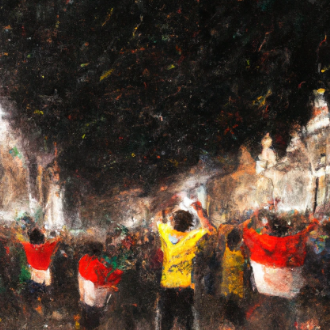
\includegraphics[width = 1.5in]{rellen_1.png} &
    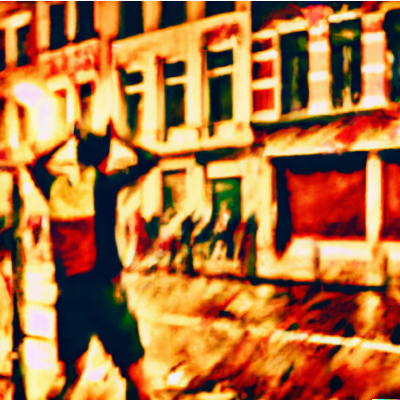
\includegraphics[width = 1.5in]{rellen_2.png} \\
    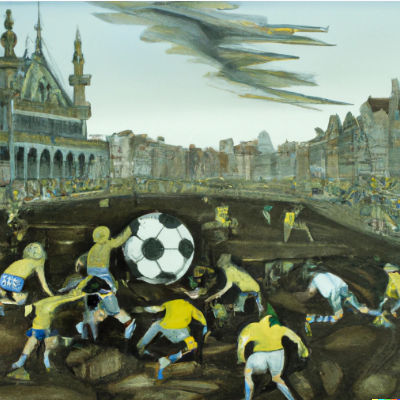
\includegraphics[width = 1.5in]{rellen_3.png} &
    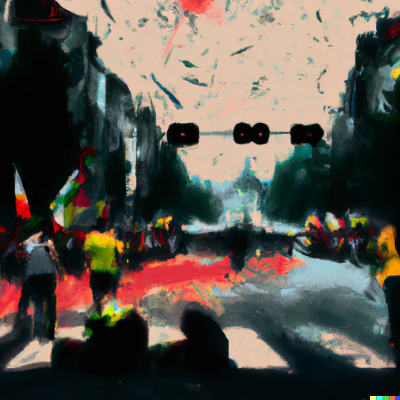
\includegraphics[width = 1.5in]{rellen_4.png}
\end{tabular} \\
\noindent
Daarnaast zal uit de turing test blijken of het kunstwerk enige boodschap overbrengt van het nieuws.
\noindent
Een voorbeeld van het resultaat van het project zou bijvoorbeeld kunnen zijn dat op een dag het hoogtepunt een artikel is over een nieuwe doorbraak in de gezondheidszorg. De applicatie zal dan op basis van de tekst van dat artikel een kunstwerk genereren dat hierbij past. In de verwachte resultaten zou dan bijvoorbeeld een afbeelding kunnen worden opgenomen van het gegenereerde kunstwerk op basis van enkele hoogtepunten van de dag. Als de gebruiker hier enige nieuws in kan herkennen en duidelijk kan verwoorden. Dan is dit een geslaagde test. 



\section*{Samenvatting}
Het doel van dit onderzoek is te onderzoeken of AI geavanceerd genoeg is om kunstwerken te genereren waarvan de boodschap herkenbaar is uit het dagelijks nieuws. In de eerste fase van het onderzoek wordt onderzocht hoe nieuwswebsites kunnen worden gescraped met behulp van de Python-library BeautifulSoup. De daaropvolgende fase omvat de verwerking van de data om de kernboodschap van de dag te identificeren. Wanneer deze is gevonden, zal deze worden gebruikt als tekstuele input om een kunstwerk te genereren met behulp van deep learning modellen, zoals Stable Diffusion of DALL-E 2, die in 2022 publiek beschikbaar zijn gesteld. Het uiteindelijke resultaat wordt beoordeeld met behulp van een turing test, om te meten of de gegenereerde kunstwerken enige boodschap of emotie oproepen die herkenbaar zijn rond het dagelijks nieuws. Dit onderzoek zal inzicht geven in de huidige staat van AI-technologieën en hun vermogen om realistische kunstwerken te genereren op basis van dagelijks nieuws, en hoe deze technologiën zich kunnen ontwikkelen in de toekomst.

%%---------- Backmatter, referentielijst ---------------------------------------

\backmatter{}

\setlength\bibitemsep{2pt} %% Add Some space between the bibliograpy entries
\printbibliography[heading=bibintoc]

\end{document}
